% Created 2016-02-22 Mon 16:55
\documentclass[11pt]{article}
\usepackage[utf8]{inputenc}
\usepackage[T1]{fontenc}
\usepackage{fixltx2e}
\usepackage{graphicx}
\usepackage{grffile}
\usepackage{longtable}
\usepackage{wrapfig}
\usepackage{rotating}
\usepackage[normalem]{ulem}
\usepackage{amsmath}
\usepackage{textcomp}
\usepackage{amssymb}
\usepackage{capt-of}
\usepackage{hyperref}
\usepackage{tikz}
\usepackage{fancyhdr}
\usepackage[left=2cm,right=2cm,top=2cm,bottom=2cm]{geometry}
\renewcommand\vec{\mathbf}
\newcommand\leftidx[3]{{\vphantom{#2}}#1#2#3}
\newenvironment{example}[1]{\vspace{0.2in}\hrule\vspace{0.1in}\noindent\emph{Example:} #1 \\}{\vspace{0.1in}\hrule\vspace{0.2in}}
\pagestyle{fancyplain}
\cfoot{{\it ENGY 5050, Nuclear Reactor Physics, UMass Lowell}}
\author{Justin Pounders}
\date{\today}
\title{ENGY 5050}
\hypersetup{
 pdfauthor={Justin Pounders},
 pdftitle={ENGY 5050},
 pdfkeywords={},
 pdfsubject={},
 pdfcreator={Emacs 24.5.1 (Org mode 8.3.2)}, 
 pdflang={English}}
\begin{document}

\maketitle
\tableofcontents


\section{Neutron-Nucleus Reactions}
\label{sec:orgheadline13}
\subsection{Introduction}
\label{sec:orgheadline1}
A neutron striking a nucleus may elicit a number of different reactions.  The types of reactions may be broadly divided into \emph{absorption} and \emph{scattering} reactions.  Absorption reactions are those in which the neutron is integrated into the nucleus, forming a new nucleus.  Normally this results in an excited, unstable nucleus.  The most common way for the nucleus to alleviate the pressure of the new nucleon is through emission of a photon.  The neutron never re-emerges, so this type of reaction is called a \emph{capture} reaction.  For fissile isotopes, the absorption process normally causes the nucleus to split violently into two pieces, or in other words, \emph{fission}.

Scattering-type reactions can be broadly divided into two categories: \emph{elastic} and \emph{inelastic}.  Elastic scattering may be viewed as a classical collision between two solid, non-deformable objects.  Billiard balls are the prototypical example.  Because neither object is "deformed" or excited, energy and linear momentum are conserved in the system.  This is in contrast to inelastic collisions.  

In inelastic scattering reactions, the neutron is actually temporarily absorbed into the nucleus, bringing the nucleus to a compound, excited state.  The compound nucleus then relaxes by emitting both a neutron \emph{and} a photon within a small fraction of a second.  The absorption-reemission process is so fast (with respect to all other time scales of neutron transport) that it may safely be regarded as instantaneous.  Because of the photon emission, neither the kinetic energy nor the momentum of the neutron-nucleus system is conserved.

Nuclear interactions are typically labeled by identifying the target nucleus, the incoming projectile/particle, particles emitted after the reaction, and the nucleus remaining when the dust settles.  For example, given a nucleus \(A\) that is struck by a particle \(p\) leading to the emission of particle \(q\) and a new nucleus \(B\) one would write \(A(p,q)B\).  If the nuclei \(A\) and \(B\) are implicitly assumed then we may simply identify the reaction as a \((p,q)\) reaction.  Thus our reaction hierarchy so far may be written as

\begin{itemize}
\item Absorptions
\begin{itemize}
\item Capture, \((n,\gamma)\)
\item Fission, \((n,f)\)
\end{itemize}
\item Scattering
\begin{itemize}
\item Elastic scattering, \((n,n)\)
\item Inelastic scattering, \((n,n')\)
\end{itemize}
\end{itemize}

Note that we have abused the original notation somewhat (this is standard) by writing \(f\) in place of an ejected particle to denote fission.  We have also written \(n'\) as the ejected particle in inelastic scattering as a reminder that the ejected particle will in general \emph{not} be the same neutron that struck the nucleus.  In some cases, high-energy inelastic scattering reactions may in fact yield more than one neutrons, in which would be denoted \((n,2n)\), \((n,3n)\), etc. with no apostrophe on the ejected particles.

\subsection{Scattering Reactions}
\label{sec:orgheadline9}
To describe the kinematics of neutron-nucleus scattering we will begin with several assumptions.
\begin{enumerate}
\item Relativistic effects can be neglected.  The kinetic energies of neutrons emitted from fission are low enough so that the space-time effects described by relativity may be neglected.
\item Neutron-neutron interactions will be neglected.  Because the density of nuclei in a reactor is much higher than the density of neutrons, neutrons are much more likely to collide with nuclei than they are with other neutrons.
\item Neutrons travel in straight lines between collisions.  This assumption holds because neutrons are neutrally-charged particles and the effect of gravity on neutron trajectories is negligible.
\item Reactors materials are isotropic.  This means that a material has no preferred orientation.  On the scale of neutron-nucleus interactions in a reactor this is a valid assumption.
\end{enumerate}

\subsubsection{Scattering Kinematics}
\label{sec:orgheadline2}

Let us now consider the specific kinematics associated with scattering.
\begin{description}
\item[{\(\vec{V}_n\), \(\vec{V}_n'\) :}] initial and final velocity of the neutron.
\item[{\(E\), \(E'\) :}] initial and final kinetic energy of the neutron.
\item[{\(\vec{V}_A\), \(\vec{V}_A'\) :}] initial and final velocity of the nucleus.
\end{description}
We also define the angles \(\gamma\), \(\theta\), and \(\psi\) as shown in Figure \ref{fig::scatteringLAB}.

\begin{figure}
\centering
\begin{tikzpicture}[x=0.25in,y=0.25in,scale=0.75]
  \draw (3,0) circle [radius=1];
  \draw (3,0) node {\large n};
  \draw [->,thick] (4.5,0) -- (9.5,0);
  \draw (7.25,1) node {$\vec{V}_n$};

  \draw (15,-5) circle [radius=2];
  \draw (15,-5) node {\huge A};
  \draw [->,thick] (13,-3) -- (10.5,-0.5);
  \draw (11,-2) node {$\vec{V}_A$};

  \draw[dashed] (10,0) -- (18,0);

  \draw (12,0) arc [start angle=0, end angle=-45, radius=2];
  \draw (12.3,-1) node {$\gamma$};

  \draw (15.77,-12.11) circle [radius=1];
  \draw (15.77,-12.11) node {\large n};
  \draw [<-,thick] (14.5,-12.75) -- (10,-15);
  \draw (11.75,-13) node {$\vec{V}_n$};

  \draw (14.87,-18.25) circle [radius=2];
  \draw (14.87,-18.25) node {\huge A};
  \draw [<-,thick] (13,-17) -- (10,-15);
  \draw (11,-16.5) node {$\vec{V}_A$};

  \draw[dashed] (2,-15) -- (18,-15);

  \draw (12,-15) arc [start angle=0, end angle=-33.69, radius=2];
  \draw (12.34,-15.7) node {$\psi$};

  \draw (11.5,-15) arc [start angle=0, end angle=26.57, radius=1.5];
  \draw (12.3,-14.4) node {$\theta$};
\end{tikzpicture}
\caption{Neutron-nucleus collision in LAB coordinates.}
\label{fig::scatteringLAB}
\end{figure}

The analysis of scattering kinematics is greatly simplifed by working in the center-of-mass reference frame (CM) rather than the laboratory reference frame (LAB).  The origin in the CM reference frame is 
\begin{align}
  \vec{r}_{CM} = \frac{1}{A+1} \left( \vec{r}_n + A\vec{r}_A \right)
\end{align}
where \(\vec{r}_n\) and \(\vec{r}_A\) are the positions of the neutron and the nucleus, respectively, and \(A\) is the atomic mass ratio of the nucleus (i.e., the ratio of the mass of the nucleus to the mass of the neutron).  Consequently we may deduce that the origin of the CM system is moving with a velocity of
\begin{align}
  \vec{V}_{CM} = \frac{1}{A+1} \left(\vec{V}_n + A\vec{V}_A \right).
\end{align}

The velocities of the neutron and nuclear in the CM system are given by the following relations:
\begin{subequations}
\begin{align}
  \vec{v}_n  &= \vec{V}_n - \vec{V}_{CM} \\
  \vec{v}_n' &= \vec{V}_n' - \vec{V}_{CM} \\ 
  \vec{v}_A  &= \vec{V}_A - \vec{V}_{CM} \\
  \vec{v}_A' &= \vec{V}_A' - \vec{V}_{CM}
\end{align}
\label{eq:cmDefs}
\end{subequations}
We will also define the \emph{relative} velocity between the neutron and nucleus, which is the same in both the CM and LAB systems:
\begin{align}
  \vec{V}_R = \vec{V}_n - \vec{V}_A
\end{align}
This definition allows us to write the CM neutron and nucleus velocities as
\begin{subequations}
\begin{align}
  \vec{v}_n = \frac{A}{A+1}\vec{V}_R \\
  \vec{v}_A = \frac{-1}{A+1}\vec{V}_R
\end{align}
\label{eq:cmVelRel}
\end{subequations}
Thus in the CM system, both neutron and nucleus are moving along the same line in opposite directions before the collision, as shown in Figure \ref{fig::scatteringCM}.

\begin{figure}
\centering
\begin{tikzpicture}[x=0.25in,y=0.25in,scale=0.75]
  \draw (3,0) circle [radius=1];
  \draw (3,0) node {\large n};
  \draw [->,thick] (4.5,0) -- (9.5,0);
  \draw (7.25,1) node {$\vec{v}_n$};

  \draw (15.5,0) circle [radius=2];
  \draw (15.5,0) node {\huge A};
  \draw [->,thick] (13,0) -- (10.5,0);
  \draw (12,1) node {$\vec{v}_A$};


  \draw (15.77,-10.11) circle [radius=1];
  \draw (15.77,-10.11) node {\large n};
  \draw [<-,thick] (14.5,-10.75) -- (10,-13);
  \draw (11.75,-11) node {$\vec{v}_n'$};

  \draw (5.3,-15.35) circle [radius=2];
  \draw (5.3,-15.35) node {\huge A};
  \draw [<-,thick] (7.3,-14.34) -- (10,-13);
  \draw (9.8,-14.2) node {$\vec{v}_A'$};

  \draw[dashed] (2,-13) -- (18,-13);

  \draw (11.5,-13) arc [start angle=0, end angle=26.57, radius=1.5];
  \draw (12.3,-12.4) node {$\varphi$};
\end{tikzpicture}
\caption{Neutron-nucleus collision in CM coordinates.}
\label{fig::scatteringCM}
\end{figure}

Consider now the kinetic energy of the system before the collision.  Letting the variable, \(e\), denote the kinetic energy of a particle in the CM system (i.e., relative to the CM velocity) we  have
\begin{align}
  e_n + e_A = e_{\text{exc}}
\end{align}
where the subscripts are used in the same way as they were in the velocity variables.  The new variable \(e_{\text{exc}}\) is called the \emph{excitation energy}, which is the energy that is available for the reaction, and may be written
\begin{align}
  e_{\text{exc}} = \frac{1}{2} \frac{mA}{A+1}V_R^2
\end{align}
where \(m\) is the mass of a neutron.

\subsubsection{Elastic Scattering}
\label{sec:orgheadline4}
We will now assume that linear momentum is conserved through the collision.  In the LAB system this means
\begin{align}
  \vec{V}_n + A\vec{V}_A = \vec{V}_n' + A\vec{V}_A'
\end{align}
By using the definitions in Eq. \eqref{eq:cmDefs} we see that this relationship carries over to CM system, allowing us to write
\begin{align}
  \vec{v}_n + A\vec{v}_A = \vec{v}_n' + A\vec{v}_A'
\end{align}
Writing the left-hand-side of this expression (i.e., the pre-collision linear momentum) in terms of the relative velocity reveals that net linear momentum both before and after the collision is zero:
\begin{align}
  \frac{A}{A+1}\vec{V}_R - \frac{A}{A+1}\vec{V}_R = \vec{0}
\end{align}
This means that
\begin{align}
  \vec{v}_n = -A \vec{v}_A, \\
  \vec{v}_n' = -A \vec{v}_A'.
\end{align}

Let us now additionally assume conservation of kinetic energy before and after the collision.  That is, 
\begin{align}
  e_n + e_A = e_n' + e_A' = e_{\text{exc}}.
\end{align}
Using Eq. \eqref{eq:cmVelRel}, we find that 
\begin{align}
  v_n = v_n' = \frac{A}{A+1}V_R,
\end{align}
and
\begin{align}
  v_A = v_A' = \frac{1}{A+1}V_R.
\end{align}

\paragraph{Stationary Target Nucleus}
\label{sec:orgheadline3}
Consider the special case where target nucleus is stationary, i.e. \(\vec{V}_A = 0\).  From the previous section we know that
\begin{align}
  \vec{V}_{CM} = \frac{1}{A+1} \vec{V}_n, \text{ and} \\
  v_n = v_n' = \frac{A}{A+1}V_n.
\end{align}
We can sketch a diagram of the relationship between the LAB and CM velocities and the velocity of the center-of-mass.

\begin{figure}
\centering
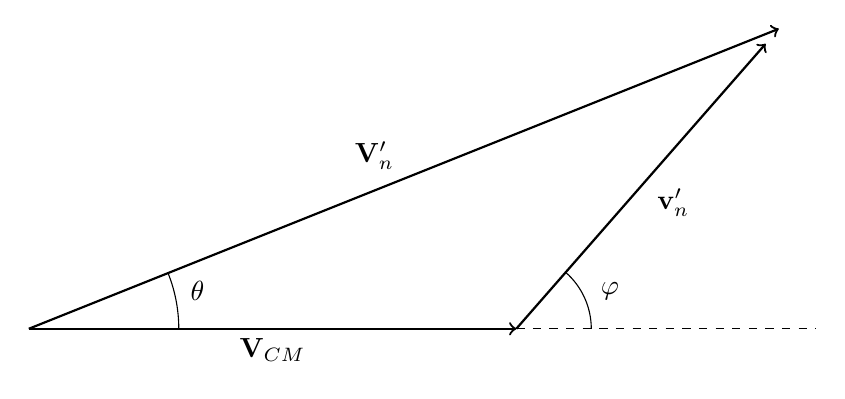
\begin{tikzpicture}[x=0.25in,y=0.25in,scale=0.75]
  \draw [->,thick] (0,0) -- (13,0);
  \draw (6.5,0) node[anchor=north] {$\vec{V}_{CM}$};

  \draw [->,thick] (0,0) -- (20,8);
  \draw (10,4) node[anchor=south east] {$\vec{V}_n'$};

  \draw [->,thick] (13,0) -- (19.65,7.6);
  \draw (16.5,4) node[anchor=north west] {$\vec{v}_n'$};

  \draw [dashed] (13,0) -- (21,0);

  \draw (15,0) arc [start angle=0, end angle=48.84, radius=2];
  \draw (15.5,1) node {$\varphi$};

  \draw (4,0) arc [start angle=0, end angle=21.8, radius=4];
  \draw (4.5,1) node {$\theta$};
\end{tikzpicture}
\caption{Relationship between final neutron velocities in LAB and CM.}
\label{fig::scatteringVelLABvsCM}
\end{figure}

From this diagram, we can apply the law of cosines to find
\begin{equation}
  V_n'^2 = V_{CM}^2 + v_n'^2 + 2 V_{CM}v_n'\cos(\pi-\varphi)
\end{equation}
which simplifies to
\begin{equation}
  V_n'^2 = \left[ \frac{A^2+1}{(A+1)^2} + 2 \frac{A}{(A+1)^2}\cos(\varphi) \right] \vec{V}_n^2.
\end{equation}
An immediate implication of this expression is the relationship between the final and initial kinetic energies of the neutron and the scattering angle in the CM system:
\begin{align}
  \frac{E_n'}{E_n} = \frac{V_n'^2}{\vec{V}_n^2}
                   = \frac{(1+\alpha) + (1-\alpha) \cos(\varphi)}{2}
\end{align}
where
\begin{align}
  \alpha = \left( \frac{A-1}{A+1} \right)^2
\end{align}

To understand this a bit better let's consider a few limiting cases.
\begin{description}
\item[{\(A=1\) :}] This is the case of a neutron scattering off a hydrogen nucleus, and \(\alpha = 0\).  For a glancing collision, the angle of deflect (\(\varphi\) or \(\theta\)) will be very small.  Thus \(E_n' \approx E_n\) and no appreciable energy is lost in the collision.  For a direct hit, in which case the neutron bounces straight back (\(\varphi = \theta = \pi\)) we have \$E\(_{\text{n}}\)' = 0\$--the neutron lost \emph{all} of its energy in a single collision.
\item[{\(A>>1\) :}] In this case the neutron hits something big, and \(\alpha \approx 1\).  Under these circumstances \(E_n' \approx E_n\) \emph{regardless} of the deflection angle.  Think of throwing a tennis ball against a brick wall.
\end{description}

Another important ramification is that for any fixed size of the target nucleus, \(A\), their is a limited range of possible final energies for the neutron.  The largest energy loss will occur when the neutron is scattered directly backward, in which case \(E_n' = \alpha E_n\).  On the other hand, for a small-angle glancing collision, the final energy will be only slightly less than the initial energy and \(E_n' \approx E_n\).  Note that under our current assumptions (namely, that the target nucleus is stationary) the neutron will never \emph{gain} energy.

The preceding work shows us that the amount of energy lost by a neutron depends on the mass of the target nucleus and the cosine of the deflection angle in the CM system.  We can derive a similar relationship between the energy loss and the cosine of the deflection angle in the LAB system, which is often more useful from simulation perspective.

Again starting with the diagram and using the law of cosines we have
\begin{align}
  v_n'^2 = V_n'^2 + V_{CM}^2 - 2 V_n' V_{CM} \cos\theta.
\end{align}
This simplifies to 
\begin{align}
  \left( \frac{A}{A+1} \right)^2 V_n^2 = V_n'^2 + \left( \frac{1}{A+1} \right)^2 V_n^2 - \frac{2}{A+1} V_n' V_n \cos\theta.
\end{align}
Multiplying by the mass of a neutron squared divided by four (to get an expression in terms of energies) and solving for \(\cos\theta\) yields
\begin{align}
  \cos\theta = \frac{1}{2}\left( A+1 \right) \sqrt{\frac{E_n'}{E_n}}
             - \frac{1}{2}\left( A-1 \right) \sqrt{\frac{E_n}{E_n'}}.
\end{align}

\subsubsection{Reactions Involving a Compound Nucleus}
\label{sec:orgheadline5}
Elastic scattering may be viewed a billiard ball collision.  The neutron and nucleus exchange kinetic energy and linear momentum but nothing else.  In collisions such as inelastic scattering, neutron capture, and fission however, the neutron and nucleus combine to form a new, compound nucleus.  Moreover, this compound nucleus will generally be in an \emph{excited} state, having received additional internal energy from the collision.  We may write such a reaction as
\begin{align}
  \leftidx{^A_Z}{X}{} + \leftidx{^1_0}{n}{} 
  \rightarrow \leftidx{^{A+1}_Z}{X}{^*}
\end{align}
where the * symbol is used to indicate an excited state.  The first reaction in this process is the absorption of a neutron into the target nucleus.  The resultant excited nucleus will then decay, generally on a time scale of \(10^{-14}\) to \(10^{-21}\) seconds.

There are two sources of the excitation energy in a compound nucleus.  First, there is the kinetic energy that is available to the reaction.  This energy, \(e_{\text{exc}}\), is the total pre-collision kinetic energy of the neutron and nucleus in the CM reference frame.  Second, there is a potential source of energy arising from the change in binding energy between the original and compound nuclei.  This change in energy may be expressed as
\begin{align}
  \Delta BE = \left[ M(A,z) + m_n - M(A+1,Z) \right] c^2
\end{align}
where \(M(A,Z)\) is the mass of nucleus \(\leftidx{^A_Z}{X}{}\), \(m_n\) is the mass of the neutron and \(c\) is the speed of light in a vacuum.  Thus the total energy available to the reaction is \(e_{\text{exc}} + \Delta BE\).

Figure \ref{fig::compoundNucleus} shows a cartoon depicting the excitation of a nucleus following neutron capture and three possible de-excitation processes (also called \emph{decay channels}).  Elastic scattering has already been discussed, and as we will see, can be treated as a special case of inelastic scattering, which we will now discuss.
\usetikzlibrary{decorations.pathmorphing}
\begin{figure}
\centering
\begin{tikzpicture}[x=0.25in,y=0.25in,scale=0.75]
  \draw (17,0) node [anchor=north] {$\leftidx{^{A+1}_Z}{X}{}$};
  \draw (14,0) -- (20,0);
  \draw (14,6) -- (20,6);
  \draw (14,11) -- (20,11);
  \draw (14,15) -- (20,15);
  \draw (14,18) -- (20,18);
  \draw (14,20) -- (20,20);
  \draw (14,22) -- (20,22);
  \draw (14,23.5) -- (20,23.5);
  \draw (14,0) -- (14,25);
  \draw (20,0) -- (20,25);

  \draw (7,17) node [anchor=north] {$\leftidx{^A_Z}{X}{}$};
  \draw (4,17) -- (10,17);
  \draw (4,21) -- (10,21);
  \draw (4,24) -- (10,24);
  \draw (4,17) -- (4,25);
  \draw (10,17) -- (10,25);

  \draw [dashed] (14,23.5) -- (0,23.5);
  \draw [dashed] (20,17) -- (0,17);
  \draw [dashed] (14,0) -- (0,0);

  \draw [<->,thick] (2,0) -- (2,17);
  \draw (2,8.5) node [fill=white] {$\Delta BE$};

  \draw [<->,thick] (2,17) -- (2,23.5);
  \draw (2,20.25) node [fill=white] {$e_\text{exc}$};

  \draw [->,thick] (15,23.5) -- (6,21);
  \filldraw [fill=white, draw=black] (12,22.6) circle [radius=0.15in];
  \draw (12,22.6) node {1};

  \draw [->,thick] (16,23.5) -- (8,17);
  \filldraw [fill=white, draw=black] (12,20.25) circle [radius=0.15in];
  \draw (12,20.25) node {2};

  \draw [->,decorate,decoration={snake}] (6,21) -- (6,17);
  \draw [->,decorate,decoration={snake}] (17,23.5) -- (17,15);
  \draw [->,decorate,decoration={snake}] (18,23.5) -- (18,11);
  \draw [->,decorate,decoration={snake}] (19,23.5) -- (19,6);
  \filldraw [fill=white, draw=black] (17.8,10) circle [radius=0.15in];
  \draw (17.8,10) node {3};

  \draw [->] (22,0) -- (22,4);
  \draw (22,2) node [anchor=west] {$E$};
\end{tikzpicture}
\caption{Formation of a compound nucleus following neutron capture.  The decay channels shown are \textcircled{1} inelastic scattering, \textcircled{2} elastic scattering, and \textcircled{3} radiative capture.}
\label{fig::compoundNucleus}
\end{figure}

\subsubsection{Inelastic Scattering}
\label{sec:orgheadline6}
Inelastic scattering involves the formation of a compound nucleus which subsequently decays through the emission of a neutron and one or more photons (\(\gamma\) rays):
\begin{align}
  \leftidx{^A_Z}{X}{} + \leftidx{^1_0}{n}{} 
  \rightarrow \leftidx{^{A+1}_Z}{X}{^*}
  \rightarrow \leftidx{^A_Z}{X}{} + \leftidx{^1_0}{n}{} + \gamma
\end{align}
The presence of the photon at the end of this reaction clearly indicates that energy has not been conserved between the neutron-nucleus pair.  What has happened instead, is that upon ejection of the neutron, the \(\leftidx{^A_Z}{X}{}\) was actually left in an excited state and emitted one (or more) photons to return to the ground state.

When considering the energetics of inelastic scattering, note that the final nucleus is simply the original target nucleus.  Thus the role of the change in binding energy has no net effect on the energy of the system.  There was \(e_\text{exc}\) energy available before the collision (from the kinetic energy of the neutron and nucleus) and there is still \(e_\text{exc}\) energy available after the collision, although the photon has appeared and claimed part of the available energy.

A second consideration is that for the compound nucleus to decay into an excited state, there must have been at least enough energy, \(e_\text{exc}\), to bridge the gap between the ground and the first excited state of the original nucleus.  Otherwise there would not have been enough energy available after the neutron emission for the target nucleus to be in an excited state!  This type of reaction is known as a \emph{threshold} reaction, because the energy of the colliding pair must meet a certain "threshold" value before the reaction can take place.  Note that if the compound nucleus emits a neutron and returns the target nucleus to its ground state, then there is no photon emission (which is only a result of de-excitation), thus the total energy of the reaction \(e_\text{exc}\) is shared between the neutron and nucleus as kinetic energy.  This, however, implies overall conservation of kinetic energy between the neutron and nucleus, thus it is an \emph{elastic} scattering event!

\subsubsection{Radiative Capture}
\label{sec:orgheadline7}
A radiative capture reaction is essentially an inelastic neutron scattering \emph{without the neutron}.  That is, the target nucleus absorbs a neutron then de-excites simply by emitting one or more photons:
\begin{align}
  \leftidx{^A_Z}{X}{} + \leftidx{^1_0}{n}{} 
  \rightarrow \leftidx{^{A+1}_Z}{X}{^*} + \gamma
\end{align}
Note that the total amount of energy to be relieved through the emission of photons is \(e_{\text{exc}} + \Delta BE\).

\subsubsection{Fission Reactions}
\label{sec:orgheadline8}
In a fission reaction, the energy \(e_{\text{exc}} + \Delta BE\) is enough to overcome the fission barrier (which is an energy threshold), and the nucleus splits into two fragments plus several free neutrons and photons.  The nuclear configuration of the fission fragments and the number of free neutrons emitted are both statistical quantities.  
\subsection{References}
\label{sec:orgheadline10}
\begin{itemize}
\item \href{Hebert2009}{Hebert}
\item \href{Duderstadt:Hamilton1976}{Duderstadt and Hamilton}
\item \href{Stacey2001}{Stacey}
\end{itemize}
\subsection{Problems}
\label{sec:orgheadline11}
\begin{enumerate}
\item In the formation of a compound nucleus, why is the available energy equal to \(e_\text{exc}\), the energy in the CM system, rather than the total kinetic energy in the LAB system?
\item Show that conservation of linear momentum in the LAB system implies conservation of linear momentum in the CM system.
\item Show that conservation of energy in the LAB system implies conservation of energy in the CM system.
\end{enumerate}
\subsection{Solutions}
\label{sec:orgheadline12}
\begin{enumerate}
\setcounter{enumi}{1}
\item Starting with conservation of momentum in the in the LAB system we have
\begin{align}
  \vec{V}_n + A \vec{V}_A = \vec{V}_n' + A \vec{V}_A'.
\end{align}
Substituting in the CM velocity definitions provides
\begin{align}
  \vec{v}_n + A \vec{v}_A + (1+A) \vec{V}_{CM} = \vec{v}_n' + A \vec{v}_A' + (1+A) \vec{V}_{CM}.
\end{align}
Canceling the CM velocity terms yields conservation of momentum in the CM system.
\item Starting with conservation kinetic energy in the LAB system we have
\begin{align}
  \frac{1}{2} m V_n^2 + \frac{1}{2}mA V_A^2 = \frac{1}{2} m (V_n')^2 + \frac{1}{2}mA (V_A')^2 
\end{align}
From the CM velocity definitions we have
\begin{align}
  V_n^2 &= \left| \vec{v}_n + \vec{V}_{CM} \right|^2 \\
        &= \left( v_n \cos\theta_n + V_{CM} \cos\theta_{CM} \right)^2 +
           \left( v_n \sin\theta_n + V_{CM} \sin\theta_{CM} \right)^2 \\
        &= \left( v_n^2 \cos^2\theta_n + 2 v_n V_{CM} \cos\theta_n \cos\theta_{CM} + V_{CM}^2 \cos^2\theta_{CM} \right) + \\
        &\phantom{=} \left( v_n^2 \sin^2\theta_n + 2 v_n V_{CM} \sin\theta_n \sin\theta_{CM} + V_{CM}^2 \sin^2\theta_{CM} \right) \\
        &= v_n^2 + V_{CM}^2 + 2 v_n V_{CM} \cos(\theta_n-\theta_{CM})
\end{align}
and a similar expression for \(V_A^2\).  The angles \(\theta_n\) and \(\theta_{CM}\) are the angles associated with the \(\vec{v}_n\) and \(\vec{V_{CM}}\) vectors, respectively.  Substituting these expressions into the energy balance equation yields
\begin{align}
  \frac{1}{2} m (v_n^2 + V_{CM}^2 + 2 v_n V_{CM} \cos(\theta_n-\theta_{CM})) 
+ \frac{1}{2}mA (v_A^2 + V_{CM}^2 + 2 v_A V_{CM} \cos(\theta_A-\theta_{CM})) \\
= \frac{1}{2} m (v_n'^2 + V_{CM}^2 + 2 v_n' V_{CM} \cos(\theta_n'-\theta_{CM}))
+ \frac{1}{2}mA (v_A'^2 + V_{CM}^2 + 2 v_A' V_{CM} \cos(\theta_A'-\theta_{CM})) 
\end{align}
which becomes
\begin{align}
  \frac{1}{2} m (v_n^2 + 2 \vec{v}_n \cdot \vec{V}_{CM} ) 
+ \frac{1}{2}mA (v_A^2 + 2 \vec{v}_A \cdot \vec{V}_{CM}) \\
= \frac{1}{2} m (v_n'^2 + 2 \vec{v}_n' \cdot \vec{V}_{CM})
+ \frac{1}{2}mA (v_A'^2 + 2 \vec{v}_A' \cdot \vec{V}_{CM}) .
\end{align}
We know that \(\vec{v}_n = -A \vec{v}_A\) and \(\vec{v}_n' = -A \vec{v}_A'\), so we have
\begin{align}
  \frac{1}{2} m v_n^2
+ \frac{1}{2}mA v_A^2
= \frac{1}{2} m v_n'^2
+ \frac{1}{2}mA v_A'^2,
\end{align}
which is the conservation of energy in the CM.
\end{enumerate}

\section{Cross Sections}
\label{sec:orgheadline27}
\subsection{What is a Cross Section?}
\label{sec:orgheadline14}
We have already assumed that neutrons travel along straight trajectories between collisions and argued that this is indeed a valid assumption within studies of nuclear reactor physics.  But how can we characterize the frequency of collisions for neutrons traveling along a given trajectory?  Put another way, if a neutron starts along a trajectory from a known point, how long should we expect it to travel before it experiences a collision.  This is clearly a problem for probability.  Hebert (2009) summarizes the problem nicely.

\begin{quote}
The probablity for a neutron located at \(\vec{r}\) and moving in a material at velocity \(\vec{V}_n\) to undergo a nuclear reaction in a differential element of trajectory \(ds\) is independent of the past history of the neutron and is proportional to \(ds\).
\end{quote}

In concrete terms, let's say that we have a  neutron that starts moving at a fixed velocity a medium  containing a exactly one kind of nucleus.  Then define \(P[ds]\) as the probability that the neutron will experience a collision within a differential distance \(ds\), and consider the following
\begin{itemize}
\item We were told (above) that the probability \(P[ds]\) is proportional to \(ds\).
\item From intuition, we can also convince ourselves that this probability should also be proportional to the number of "target" nuclei present, so let's define \(N\) as the density of nuclei.
\end{itemize}
From these observations we may write
\begin{align}
  P[ds] = \sigma N ds
\end{align}
The quantity \(P[ds]\) is a probability, so it should be unitless.  Given that \(N\) is a density and \(ds\) is length, we can infer that the proportionality constant, \(\sigma\), has units of length squared or area.  The constant \(\sigma\) is called the \emph{microscopic cross section}.  It is common to express the microscopic cross section in units of \emph{barns} (b) where \(1 \text{ b} = 10^{-24} \text{ cm}^2\).

The product of the first two variables appearing on the right-hand-side of the probability definition is called the \emph{macroscopic cross section}, written as
\begin{align}
  \Sigma = \sigma N,
\end{align}
which may be interpreted as the probability \emph{per unit path-length} of a collision.  Thus we may write the probability of a neutron collision over the differential path-length \(ds\) as
\begin{align}
  P[ds] = \Sigma ds.
\end{align}

Next, consider a \emph{population} of neutrons with a density, \(n\).  For now let's assume that all neutrons have the same speed, but they need not be moving in the same direction.  The number of neutrons that will experience a collision within the differential path-length \(ds\) along each of their individual trajectories will be \(P[ds]\) multiplied by the number of neutrons.  If we multiply by the \emph{density} of neutrons rather than the \emph{number} of neutrons then we get the (differential) density of neutron collisions within a (differential) distance \(ds\) of collective neutron travel:
\begin{align}
  dC = \Sigma n ds.
\end{align}
Note the units of (collisions) per unit volume.

Because all neutrons are moving at the same speed, \(V_n\), we may relate the distance \(ds\) (of "collective neutron travel") to a time interval \(dt = \frac{ds}{V_n}\).  Thus the density of neutron collisions is \(dC = \Sigma n V_n dt\).  Dividing by \(dt\) and taking \(dt \rightarrow 0\) gives us an important quantity in reactor physics, called the \emph{reaction rate density}:
\begin{align}
  R = \frac{dC}{dt} = \Sigma n V_n.
\end{align}
Because we have officially taken the limit \(dt \rightarrow 0\) (and correspondingly \(ds \rightarrow 0\)), this quantity is a point-wise, instantaneous value.

The product of neutron density and neutron speed, \(n V_n\), appearing on the right-hand-side of the reaction rate density is a ubiquitous quantity in reactor physics, called the \emph{scalar flux}:
\begin{align}
  \phi = n V_n.
\end{align}

We have previously established that there are several different types of nuclear reactions (radiative capture, elastic and inelastic scattering, etc.)  Each type of reaction is represented by unique microscopic cross section.  For a reaction of type \(x\), for example, we may write the corresponding cross section \(\sigma_x\).  Multiplying by the nuclide density provides the corresponding macroscopic cross section \(\Sigma_x = N \sigma_x\).

If there is more than one type of nuclide present, we may simply add the contributions from each to obtain macroscopic cross section for the mixture:
\begin{align}
  \Sigma_x = \sum_i N_i \sigma_{x,i}.
\end{align}
More over we may sum across all reaction types to obtain the \emph{total} macroscopic cross sections, which is the probability per unit path-length of \emph{any} collision:
\begin{align}
  \Sigma = \sum_x \Sigma_x.
\end{align}

\begin{example}{Derivation of Mean-Free-Path}
Now consider a monoenergetic beam of neutrons with uniform velocity $\vec{V}_n$ impinging normally on the surface of slab with a total macroscopic cross section $\Sigma$.  On average, how far will a neutron travel into the slab before experiencing its first collision?

First construct a balance equation for the uncollided neutron density as a function of $x$.  We know that the rate of neutron removal (with respect to $x$) will be the rate of neutron collisions, and there are no sources of uncollided neutrons inside the slab.  Thus,
\begin{align}
  \frac{dn}{dx} = -\Sigma n(x).
\end{align}
We can solve this equation to determine
\begin{align}
  n(x) = n(0) e^{-\Sigma x}.
\end{align}
The probability that a neutron will reach a distance $x$ without experiencing is a collision is thus
\begin{align}
  p_0(x) = \frac{n(x)}{n(0)} = e^{-\Sigma x}.
\end{align}

Next, the probability of a neutron experiencing its first collision between $x$ and $x+dx$ is the product of (1) the probability of the neutron reaching $x$ and (2) the probability of the neutron colliding between $x$ and $x+dx$:
\begin{align}
  p_c(x)dx = p_0(x) \Sigma dx = \Sigma e^{-\Sigma x} dx.
\end{align}

Finally, the average distance to first collision, which we will call $\lambda$, may be obtained by taking the integral
\begin{align}
  \lambda = \int_0^\infty x p_c(x) dx = \frac{1}{\Sigma}.
\end{align}
The quantity $\lambda$ is called the /mean-free-path/ and, for an infinite, homogeneous medium, is equal to the inverse of the total macroscopic cross section.
\end{example}

\subsection{Resonance}
\label{sec:orgheadline18}
Because of the quantum nature of reality, which is very important at the nuclear scale, a nucleus is not allowed to be excited to an arbitrary energy level.  Rather a nucleus may only sit at certain discrete energy levels, at or above its ground state.  Nuclei in excited states will seek to return to the stable ground state, typically though photon emission, although at high enough energy a neutron or even alpha particle may be emitted.  For some nuclei, the additional energy is sufficient to cause fission.  

Although each excitation level, say \(e_i\), is discrete, it's value is not precisely defined due to the Heisenberg uncertainty principle.  Rather each excited state is associated with an energy width, \(\gamma_i\), that is centered at \(e_i\) and related to the average lifetime of the excited state, \(\tau_i\) by
\begin{align}
  \gamma_i = \frac{\hbar}{\tau_i}.
\end{align}
Note that the average lifetime \(\tau_i\) is equal to the inverse of the decay constant for the excited state.

An excited, compound nucleus at excitation level \(e_i\) with width \(\gamma_i\) may have several options for de-excitation: emitting a photon, a neutron, etc., for example.  Each one of these "options" is called a \emph{decay channel}.  The energy width, \(\gamma_i\), of the excited state may be written as a sum of the widths associated with each possible decay channel:
\begin{equation}
  \gamma_i = \sum_x \gamma_{i,x},
\end{equation}
where \(x\) represents a decay channel.

A discussion of the quantum effects surrounding nucleus formation and de-excitation can quickly become quite involved.  While interesting, that discussion is beyond the objectives of our present endeavor.  Thus the following brief sections will only present a high-level summary of the things it might be good to know as nuclear \emph{engineer}.

Recall that there is \(e^* = e_{\text{exc}} + \Delta BE\) of energy available to a newly-created compound nucleus that has been struck by a neutron.  When \(e^*\) is close to an excitation level \(e_i\) of the compound nucleus--if the available reaction energy puts the compound nucleus rather precisely into an excited state--then we observe a \emph{resonance} condition.  A resonance condition means that is \emph{very likely} that the compound nucleus will be formed at the excited state corresponding to the \(e_i\) level.  Resonance conditions have a significant impact on the likelihood that a reaction will take place, and consequently the cross section for that reaction will be significantly affected.

\subsubsection{Single Level Breit-Wigner Formula}
\label{sec:orgheadline15}
There is a result from quantum mechanics that provides an expression for a reaction cross section in the vicinity of a resonance.  The formula is known as the \emph{single level Breit-Wigner Formula} (SLBW).  The "single level" qualifier belies the assumption the resonance in question is well-separated from nearby resonances.  Conversely, if two energy states are close enough together that their associated energy widths (\(\gamma_i\) \(\gamma_{i+1}\), for example) overlap, then the there will be interference effects between the two states.  This will then lead to more complex expressions for describing the corresponding resonance effects that manifest in the cross sections.

For a reaction of type \(x\) from which there are no emerging neutrons (e.g., radiative capture), the SLBW may be written
\begin{align}
  \sigma_x(e_{\text{exc}}) = \sigma_0 \frac{\gamma_{x,i}\gamma_i}{\gamma_i^2+4(e_\text{exc}-e_i)^2}
\end{align}
where
\begin{align}
 \sigma_0 &= 4\pi \lambda^2 g_J \frac{\gamma_{n,1}(e_\text{exc})}{\gamma_i},  \\
  g_J &= \frac{2J+1}{2(2I+1)}, \text{ and} \\
  \lambda &= \frac{\hbar}{\sqrt{2e_\text{exc} \left( \frac{Am}{A+1} \right)}}.
\end{align}
The quantity \(g_J\) is a statistical factor expressed in terms of the spin of the target nucleus (\(I\)) and compound nucleus (\(J\)).  The parameter \(\lambda\) is the de Broglie wavelength of the incident neutron in the CM system.

For an elastic scattering reaction, the SLBW becomes
\begin{align}
  \sigma_e(e_\text{exc}) = \sigma_p^\ell 
                         + \sigma_0 \left[ \frac{2}{\gamma_i}(e_\text{exc}-e_i) \sin 2\phi_\ell 
                                         + \frac{\gamma_{n,i}}{\gamma_i} -2 \sin^2 \phi_\ell \right] \frac{\gamma_i^2}{\gamma_i^2+4(e_\text{exc}-e_i)^2}
\end{align}
where
\begin{align}
  \sigma_p^\ell = 4\pi \lambda^2 \left( 2\ell + 1 \right) \sin^2 \phi_\ell
\end{align}
is called the \emph{potential} cross section.
In this expressions the quantity \(\ell\) is the integer \emph{angular momentum quantum number}, which enumerates several types of elastic scattering reactions:
\begin{align}
  \ell = 
  \begin{cases}
    0; & s\text{-wave interaction} \\
    1; & p\text{-wave interaction} \\
    2; & d\text{-wave interaction} \\
    \text{etc.} &
  \end{cases}
\end{align}
Most elastic scattering reactions in thermal reactors will be \(s\text{-wave}\) interactions, characterized by relatively low incident neutron energies.  Heavy target nuclei may give rise to higher-waver interactions.  The first few \(\phi_\ell\) \emph{shift factors} are given by
\begin{align}
  \phi_0 &= \frac{a}{\lambda}, \\
  \phi_1 &= \frac{a}{\lambda} - \tan^{-1} \frac{a}{\lambda}, \\
  \phi_2 &= \frac{a}{\lambda} - \tan^{-1} \frac{\frac{3a}{\lambda}}{3 - \left( \frac{a}{\lambda} \right)^2}
\end{align}
where \(a\) is the nucleus \emph{diffusion radius}, which can be thought of as the "radius of influence" of the nucleus.  (A nucleus does not have a well-defined boundary in the quantum world!)

The expressions so far have been defined with respect to the CM system.  Most of us do not live in the center-of-mass world of nuclear collision; we operate in a world that is stationary with respect to \emph{us}, i.e., the LAB system, and would prefer to work accordingly.  The excitation energy \(e_\text{exc}\) in the CM system can be converted to a LAB energy easily:
\begin{align}
  E_\text{exc} = \frac{A+1}{A}e_\text{exc} = \frac{1}{2} m_n V_R^2.
\end{align}
If we assume that the target nucleus is stationary, then \(E_\text{exc}\) is simply the initial kinetic energy of the neutron.

With regard to resonance descriptions, a resonance at \(e_i\) with a width \(\gamma_{x,i}\) for decay channel \(x\) in the CM system becomes the following in the LAB system:
\begin{align}
  E_i &= \frac{A+1}{A} e_i, \\
  \Gamma_{x,i} &= \frac{A+1}{A} \gamma_{x,i}.
\end{align}
The SLBW formulas remain valid in the LAB as long as the lowercase (CM) variables above are replaced by their uppercase (LAB) counterparts.

We will conclude this section by remarking that in the case of a resonance located at an energy \(e_{x,i}\) above the thermal energy range (i.e., >1 eV).  If we assume that that \(a/\lambda << 1\) then only \(s-\text{wave}\) interactions are important.  Then using LAB variables, the SLBW formulas become
\begin{align}
  \label{eq::simpleSLBW1}
  \sigma_x(E_\text{exc}) &=  \sigma_0 \frac{\Gamma_{x,i} \Gamma_i}{\Gamma_i^2 + 4\left(E_\text{exc} - E_i\right)^2} \\
  \label{eq::simpleSLBW2}
  \sigma_e(E_\text{exc}) &= 4\pi a^2 
         + \sigma_0 \frac{2a}{\lambda} \frac{2\Gamma_i\left(E_\text{exc} - E_i\right)}{\Gamma_i^2 + 4\left(E_\text{exc} - E_i\right)^2}
         + \sigma_0 \frac{\Gamma_{n,i} \Gamma_i}{\Gamma_i^2 + 4\left(E_\text{exc} - E_i\right)^2} \;\;.
\end{align}

\subsubsection{Limitations of SLBW}
\label{sec:orgheadline16}
The main assumption of the SLBW was that resonances were well-separated and did not interfere with one another.  In reality this assumption breaks down, especially in heavy target nuclei and high energies (\(\gtrsim 10\) keV).  There is a more accurate representation of closely-spaced resonances called the multilevel Breit-Wigner (MLBW) formula.  The complexity of this formula increases significantly.  The MLBW is, however, often used in computer codes that calculate neutron cross sections for reactor physics applications.

\subsubsection{Resonance Distributions}
\label{sec:orgheadline17}
The location and density of resonances varies by nuclide and energy.  In general both the number and density of resonances increases with larger nuclides and higher incident neutron energies.  Below 1-10 keV resonances are typically separated enough so that experimentalists can determine the location and width of the resonances. At higher energies, however, the resonances become so tightly spaced that is impossible, at present, to distinguish one from the other.  We say that these resonances are \emph{unresolved}, or lie in the \emph{unresolved resonance range}, in contrast to the \emph{resolved resonance range} at lower energies.
\subsection{Non-Stationary Nuclei}
\label{sec:orgheadline22}
In much of our initial discussion on neutron-nuclear interactions we assumed that the target nucleus was stationary (\(\vec{V}_A\)).  Short of being at absolute zero temperature, this is never the case in reality.  If the speed of the neutron is much larger than the speed of the target nucleus this ma be a good assumption, however, so our previous discussions are justified.  At neutron energies below 1 eV the random, thermal motion of the nuclei is not negligible.

\subsubsection{Averaging the Microscopic Cross Section}
\label{sec:orgheadline19}
The velocities of nuclei in thermal equilibrium is described by the Maxwell-Boltzmann probability density function,
\begin{align}
  p(\vec{V}_A) = \left( \frac{mA}{2\pi k T} \right)^\frac{3}{2} \exp\left(-\frac{mAV_A^2}{2kT}\right) 
\end{align}
where
\begin{description}
\item[{\(k\)}] is the Boltzmann constant,
\item[{\(T\)}] is the absolute temperature of the material,
\item[{\(m\)}] is the neutron mass,
\item[{\(A\)}] is the ratio of the nuclear mass to the mass of a neutron.
\item[{\(p(\vec{V}_A)d^3V_A\)}] is the probability for a nucleus to have a velocity within an interval \(d^3V_A\) of \(\vec{V}_A\).
\end{description}

We know that for a fixed neutron speed \(V_n\) the reaction rate for reaction type \(x\) is defined by
\begin{align}
  R_x = N \sigma_x(E_\text{exc}) V_R n,
\end{align}
where \(N\) and \(n\) are the densities of the nuclei and neutrons, respectively.  Note that because we are not assuming a stationary nucleus, we use the relative speed, \(V_R\), which is the speed at which the neutron is approaching the target, \(V_R = V_n - V_A\).  Also recall that the excitation energy  in the LAB is \(E_\text{exc} = \frac{A+1}{A}e_\text{exc} = \frac{1}{2}mV_R^2\) (where \(m\) is the neutron mass), so we may use \(E_\text{exc}\) and \(V_R\) interchangeably as the independent variable in the microscopic cross section.  Thus for a fixed neutron speed \(V_n\) the reaction rate depends on the speed of the target nucleus which is random.  To account for this thermal motion of the nuclei, we can calculate an average reaction rate over the probability distribution of target nuclei:
\begin{align}
  \left<R_x\right> = \int_0^\infty p(\vec{V}_A) N \sigma_x(\left| \vec{V}_n - \vec{V}_A \right|) \left| \vec{V}_n - \vec{V}_A \right| n d^3V_A \;\;,
\end{align}
where the integral is taken over each of the velocity components.  From this average reaction rate we can define a new \emph{effective} microscopic cross section averaged over the motion of the nuclei, which for neutron with speed \(V_n\) is:
\begin{align}
  \bar{\sigma}_x(V_n) = 
  \left<\sigma_x(\left| \vec{V}_n - \vec{V}_A \right|)\right> = 
  \frac{1}{V_n} \int_0^\infty p(\vec{V}_A) \sigma_x(\left| \vec{V}_n - \vec{V}_A \right|) \left| \vec{V}_n - \vec{V}_A \right| d^3V_A \;\;.
\end{align}

Plugging in the Maxwell-Boltzmann distribution into this expression yields
\begin{align}
  \bar{\sigma}_x(V_n) = 
  \frac{1}{V_n} \left( \frac{mA}{2\pi k T} \right)^\frac{3}{2}
  \int_0^{2\pi} \delta \int_0^\infty dV_{xy} V_{xy} \int_{-\infty}^\infty dV_z \exp\left(-\frac{mAV_A^2}{2kT} \right) \sigma_x(V_R) V_R \;\;.
\end{align}
The expression can be simplified somewhat without approximation.  To begin, consider the velocity of the target nucleus decomposed into a radial (\(xy\)) and axial (\(z\)) component:
\begin{align}
  \vec{V}_A = V_{xy} \cos\eta \vec{i} + V_{xy} \sin\eta \vec{j} + V_z \vec{k}
\end{align}
where \(\eta \in \left[0, w\pi\right]\), and
\begin{align}
  d^3V_A = V_{xy} d\eta dV_{xy} dV_z \;\;.
\end{align}
The primary quantity that needs to be evaluated for the averaging is the relative speed.  If we define the coordinate reference frame so that the \(\vec{k}\) unit vector is pointing in the direction of neutron travel then we have
\begin{align}
  V_R = | \vec{V}_n - \vec{V}_A | = \sqrt{V_{xy}^2  + \left(V_n - V_z\right)^2} \;\;.
\end{align}
Additionally,
\begin{align}
  V_A^2 = V_{xy}^2 + V_z^2 = V_R^2 - V_n^2 + 2V_nV_z \;\;.
\end{align}
Finally, changing the variable of integration of the first integral from \(V_{xy}\) to \(E_\text{exc}\) using the relationship
\begin{align}
  E_\text{exc} = \frac{1}{2}m\left[V_{xy}^2 + (V_n - V_z)^2\right]
\end{align}
(which requires changing the bounds of the \(V_z\) integration) and integrating over \(V_z\) yields
\begin{align}\label{eq::avgMicro}
  \bar{\sigma}_x(E) = \frac{1}{\Delta\sqrt{\pi}} \int_0^\infty dE_\text{exc} \sqrt{\frac{E_\text{exc}}{E}} \sigma_x(E_\text{exc}) 
  \left\{ \exp\left[ -\frac{A}{kT}\left(\sqrt{E_\text{exc}} - \sqrt{E} \right)^2 \right] 
         \exp\left[ -\frac{A}{kT}\left(\sqrt{E_\text{exc}} + \sqrt{E} \right)^2 \right]  \right\}
\end{align}
where
\begin{align}
  \Delta = 2 \sqrt{\frac{EkT}{A}} \quad \text{and} \quad E = \frac{1}{2}mV_n^2 \;\;.
\end{align}

\subsubsection{Averaging Resonance Cross Sections}
\label{sec:orgheadline20}
Accounting for the thermal motion of nuclei in resonance cross sections is at the heart of the \emph{Doppler broadening effect}, which is an important player in both steady-state and transient reactor analysis.  In the case of an isolated, narrow resonance above the thermal neutron energy range we can take several further steps to simplify Eq. \eqref{eq::avgMicro}.
\begin{enumerate}
\item If the neutron has a kinetic energy significantly above the average kinetic energy of the nuclei then \(E_\text{exc} \approx E\) and we may assume that \(\exp\left[-\frac{A}{kT}\left(\sqrt{E_\text{exc}} + \sqrt{E}\right)^2\right] << \exp\left[-\frac{A}{kT}\left(\sqrt{E_\text{exc}} - \sqrt{E}\right)^2\right]\).  Consequently we will take
\begin{align}
  \exp\left[-\frac{A}{kT}\left(\sqrt{E_\text{exc}} + \sqrt{E}\right)^2\right] \approx 0 \;\;.
\end{align}
\item Because we have assumed that the resonance is narrow we may assume that the peak energy, \(E_i\), is much greater than the resonance width, \(\Gamma_i\).
\item When \(E_\text{exc}\) is much different than \(E\), the first exponential term in Eq. \eqref{eq::avgMicro} will rapidly tend to a small number.  Thus we may generate a Taylor expansion of \(\left(\sqrt{E_\text{exc}} - \sqrt{E}\right)\) in \(E\) with \(E_\text{exc} = E + \varepsilon\) and \(\varepsilon << E\).
\item We assume \(s-\text{wave}\) interactions and use lab variables so that Eqs. \eqref{eq::simpleSLBW1} and \eqref{eq::simpleSLBW2} may be used.
\item Assume that \(\Gamma_{x,i}\) and \(\Gamma_i\) are constant.  (In reality there is some variation with energy.)
\end{enumerate}
Applying all of these assumptions and approximations leads to
\begin{align}
  \label{eq::dopplerSLBWx}
  \bar{\sigma}_x(E) &= \frac{1}{\Delta \sqrt{\pi}} \sigma_0(E) \frac{\Gamma_{x,i}}{2}
                      \int_{-2E_i/\Gamma_i}^\infty dv \frac{1}{1+v^2} \times \\
                    &\phantom{=}  \exp\left\{ -\frac{A}{kT} \frac{\Gamma_i^2(v-u)^2}{16E}
                                  \left[ 1 - \frac{1}{2}\left( \frac{\Gamma_i(v-u)}{2E} \right)
                                           + \frac{5}{16}\left( \frac{\Gamma_i(v-u)}{2E} \right)^2 + \hdots \right] \right\}
\end{align}
where
\begin{align}
  u = \frac{2}{\Gamma_i}\left(E - E_i\right)
  \quad \text{and} \quad
  v = \frac{2}{\Gamma_i}\left(E_\text{exc} - E_i\right) \;\;.
\end{align}
The lower integration limit can be replaced by \(-\infty\) because \(\Gamma_i << E_i\), leading to the following result:
\begin{align}
  \bar{\sigma}_x(E) = \sigma_0(E) \frac{\Gamma_{x,i}}{\Gamma_i} \psi(u,\alpha,\beta)
\end{align}
where
\begin{align}
  \psi(u,\alpha,\beta) = \frac{1}{\beta\sqrt{\pi}}
                         \int_{-\infty}^\infty dv \frac{1}{1+v^2} \exp\left\{ -\frac{(v-u)^2}{\beta^2}
                         \left[ 1 - \frac{1}{2}\alpha(v-u) + \frac{5}{16}\alpha^2(v-u)^2 + \hdots \right] \right\}
\end{align}
and
\begin{align}
  \alpha = \frac{\Gamma_i}{2E}
  \quad \text{and} \quad
  \beta = \frac{2\Delta}{\Gamma_i} \;\;.
\end{align}
This expression \(\psi(u,\alpha,\beta)\) is called the \emph{generalized Doppler psi function}.  A common simplification is to assume that \(E \simeq E_i\), in which case,
\begin{align}
  \beta = \frac{2\Gamma_D}{\Gamma_i}
\end{align}
where the \emph{Doppler width} has been defined as
\begin{align}
  \Gamma_D = 2 \sqrt{\frac{E_i kT}{A}}.
\end{align}

Using the same mathematical treatment, a similar expression can be derivied for the SLBW elastic scattering resonance formula.  The result is
\begin{align}
  \label{eq::dopplerSLBWe}
  \bar{\sigma}_e(E) = 4\pi a^2 + \sigma_0(E)\frac{2a}{\lambda}\phi(u,\alpha,\beta) + \sigma_0(E)\frac{\Gamma_{n,i}}{\Gamma_i}\psi(u,\alpha,\beta)
\end{align}
where
\begin{align}
  \phi(u,\alpha,\beta) = \frac{1}{\beta\sqrt{\pi}}
                         \int_{-\infty}^\infty dv \frac{v}{1+v^2} \exp\left\{ -\frac{(v-u)^2}{\beta^2}
                         \left[ 1 - \frac{1}{2}\alpha(v-u) + \frac{5}{16}\alpha^2(v-u)^2 + \hdots \right] \right\}
\end{align}

Let's take a moment to summarize what has been done in the preceding. We began with the microscopic cross section \(\sigma_x\) that is proportional to the probability of a neutron-nucleus interaction and depends on (equivalent) the excitation energy \(E_\text{exc}\) or the relative speed of the neutron-nucleus pair \(V_R\).  Either parameter is complicated by the fact that the nuclei are moving in essentially a random fashion, describable by the probability function \(p(\vec{V}_A)\).  At thermal equilibrium, this probability function is the Maxwell-Boltzmann distribution, so we can derive an expression for the microscopic cross section that is averaged over the thermal motion of the nuclei.  This was the main result.

Remember that the Maxwell-Boltzmann distribution is a function of the temperature of the material.  Thus as the temperature changes so will the averaged microscopic cross sections.  This phenomenon is called the \emph{Doppler broadening effect}.

The \(\phi-\psi\) Doppler functions derived in this section relied on several important assumptions that will not always hold up in reality.  When situations arise in which these functions are not appropriate one may resort to approximate numerical evaluations of Eq. \ref{eq::avgMicro} directly.  This is commonly done in practice.
\subsubsection{Other Considerations}
\label{sec:orgheadline21}
Many absorption-type cross sections (without resonances in the thermal energy range) vary as \(1/\sqrt{E}\) at low energies.  This is commonly referred to as a ``\(1/v\) energy-dependence,'' where \(v\) refers to the neutron speed.  Surprisingly, the thermal motion of nuclei does \emph{not} affect a cross sections with a \(1/v\) energy variation.  In other words, \(V_n \bar{\sigma_x}(V_n) = V_R\sigma_x(V_R)\) when \(\sigma_x(V_R) \propto V_R^{-1}\).

In stating that the thermal motion of the nuclei follow the Maxwell-Boltzmann distribution, we have implicitly assumed that all nuclei are free to move independently, effectively as molecules in a gas.  Most nuclei, however, are chemically bonded to other nuclei to form molecules.  Molecular motion, including vibration and rotation, for example, affects nuclear motion, so the preceding treatment is not strictly valid.  The primary regime where this becomes important is in neutron scattering at low energy. There are treatments to deal with molecular motion that we will not discuss.  

Arguably the most important example in reactor physics of where molecular motion effects are important is in the thermal scattering of neutrons in water.  An analysts should be aware that water cross sections, and hydrogen bound in water in particular, require special evaluations with respect to temperature.  When obtaining nuclear data for reactor physics calculation, this ``special evaluation'' normally appears as something called a \emph{thermal kernel} or \(S(\alpha,\beta)\) \emph{data} that is tabulated alongside all the other nuclear cross sections.
\subsection{Differential Scattering Cross Sections}
\label{sec:orgheadline23}
Up to this point we have considered scattering cross sections only in the sense as they relate to the probability of a scattering event taking place.  In reactor physics analysis, where we want to track the movement of neutrons through a reactor, we often need more information than this.  In particular, if a neutron scatters we want the ability to predict (in a probabilistic sense) how the scattering event will affect the neutrons energy and direction.

In general we can describe probabilistic scattering kinematics as the product of two functions.  The first is the microscopic cross section for the scattering reaction, which relates the likelihood that the scattering event occur.  We can multiply the cross section by a probability function describing the probability that, upon scattering at a certain energy \(E\), the neutron will emerge from the collision with a new energy \(E'\) and a direction modified by some angle \(\theta\).  We write this as
\begin{align}
  \sigma_n(E \rightarrow E', \mu) = \sigma_n(E)P(E \rightarrow E', \mu)
\end{align}
where \(\sigma_n(E)\) is the microscopic cross section for scattering (elastic or inelastic) and \(P(E \rightarrow E', \mu)dE'd\mu\) is the probability that the neutron will scatter to energy \(E'\) (within an interval \(dE'\) through a deviation cosine \(\mu = \cos\theta\) (within an interval \(d\mu\)).  The quantity \(\sigma_n(E \rightarrow E', \mu)\) is called the \emph{double differential scattering cross section} and is sometimes written as
\begin{align}
  \sigma_n(E \rightarrow E', \mu) \equiv \frac{d^2\sigma_n(E)}{dE'd\mu} \;\;.
\end{align}

\begin{example}{Double-Differential Elastic Scattering Cross Section, Stationary Target}
We previously saw that elastic, isotropic (in CM) scattering off a stationary target leads to the following relationship between energies $E$, $E'$, and CM scattering angle $\varphi$:
\begin{align}
  \frac{E_n'}{E_n} = \frac{V_n'^2}{\vec{V}_n^2}
                   = \frac{(1+\alpha) + (1-\alpha) \cos(\varphi)}{2}
\end{align}
where $\alpha = (A-1)^2/(A+1)^2$.  From this we see that energy and direction change are directly correlated.  The probability density function for a neutron scattering isotropically through the cone created by angle $\varphi$ is given by
\begin{align}
  P(\phi) = \frac{1}{2} \sin\varphi, \quad \phi\in[0,\pi] \;\;.
\end{align}
We see that an increase in $\varphi$ by an amount $d\varphi$ causes a decrease in the exiting energy by an mount $dE'$, and in particular,
\begin{align}
  dE' = - \frac{E(1-\alpha)\sin\varphi}{2}d\varphi \;\;.
\end{align}
Because energy change is directly related to the deviation angle we may write the following expression for the probability that a neutron will be scattered from energy $E$ to energy $E'$:
\begin{align}
  P(E \rightarrow E') dE' = - P(\varphi) d\varphi \;\;.
\end{align}
Substituting in the eliminating $d\varphi$ in favor of $dE'$, then cancelling the differential, and subsituting the expression for $P(\varphi)$ leads to
\begin{align}
  P(E \rightarrow E') = \frac{1}{E(1-\alpha)} \;\;.
\end{align}

What we really want is the probability as a function of energy /and/ angle in the LAB, but we just saw that these are correlated.  We previously derived the following results for the LAB deviation cosine in this scenario:
\begin{align}
  \mu = \cos\theta = \frac{1}{2}\left( A+1 \right) \sqrt{\frac{E_n'}{E_n}}
                   - \frac{1}{2}\left( A-1 \right) \sqrt{\frac{E_n}{E_n'}} \;\;.
\end{align}
Because energy and angle correlated, the function $P(E \rightarrow E', \mu)$ is really a one-parameter function, not two.  Thus we may write
\begin{align}
  P(E \rightarrow E', \mu) = 
  \begin{cases}
    \frac{1}{E(1-\alpha)}\delta\left( \mu - \frac{1}{2}\left( A+1 \right) \sqrt{\frac{E_n'}{E_n}}
                                     - \frac{1}{2}\left( A-1 \right) \sqrt{\frac{E_n}{E_n'}} \right), & \text{if } \alpha E \leq E' \leq E, \\
    0, & \text{otherwise.}
  \end{cases}
\end{align}
The function $\delta(x)$ is the /Dirac delta function/ (see the Appendix for details).
\end{example}

Both \(\sigma_n(E)\) and \(P(E \rightarrow E', \mu)\) depend on the thermal motion of nuclei and there are methods for averaging these quantities over that motion similar to what was shown in the previous section, but these procedures will not be discussed here as they become quite complex, even for the relatively simple case of elastic scattering.
\subsection{References}
\label{sec:orgheadline24}
\begin{itemize}
\item \href{Hebert2009}{Hebert (2009)}
\end{itemize}
\subsection{Problems}
\label{sec:orgheadline25}
\begin{enumerate}
\item In general the ratio of the diffusion radius of a nucleus (\(a\)) to the neutron wavelength (\(\lambda\)) is much less than one, i.e. \(\frac{a}{\lambda} << 1\).  Under this assumption, derive an approximate expression for the \emph{potential} elastic scattering cross section, \(\sigma_p^\ell\), for \(s\)-wave interactions.
\item Derive the Maxwell-Boltzmann distribution as a function of \emph{kinetic energy}, \(E = \frac{1}{2}mA|\vec{V}_A|^2 = \frac{1}{2} m_A V_A^2\). Start with the Maxwell-Boltzmann distribution written as a function of velocity \(\vec{V}_A\).  Because this is a \emph{distribution} the change of variables must be done so that \(p(\vec{V}_A) d^3V_A = p(E) dE\).  (Note that although \(\vec{V}_A\) is a vector, the direction of the vector is not important, as all that appears in the distribution is \(V_A^2\), which is proportional to energy.  Thus we may write \(d^3 V_A = 4\pi V_A^2 dV_A\).)
\item Plot the Maxwell-Boltzmann distribution as a function of kinetic energy using your results from the previous problem.  Use \(T = 300\) K.  Does this plot inform the reasoning behind picking an energy of around 1 eV as the cutoff for ``thermal'' neutron energies?
\item Derive Eqn. \ref{eq::dopplerSLBWx}.
\end{enumerate}
\subsection{Solutions}
\label{sec:orgheadline26}
\begin{enumerate}
\item The potential elastic scattering cross section is given by
\begin{align}
  \sigma_p^\ell = 4\pi \lambda^2 \left(2 \ell + 1 \right) \sin^2\phi_\ell.
\end{align}
For an \(s\)-wave interaction \(\ell = 0\), and \(\phi_0 = a/\lambda\).  Because \(a/\lambda << 1\) we can use the small-angle approximation for sine: \(\sin\theta \approx \theta\) for \(|\theta| << 1\).  Plugging \(\ell\) and \(\phi_\ell\) into the equation and using the small-angle approximation leads
\begin{align}
  \sigma_p^0 = 4\pi a^2.
\end{align}
Note that this is the surface area of a sphere with radius \(a\).
\item Begin with 
\begin{align}
  p(\vec{V}_A) = \left( \frac{m_A}{2\pi k T} \right)^\frac{3}{2} \exp\left(-\frac{m_A V_A^2}{2kT}\right) .
\end{align}
and \(d^3 V_A = 4\pi V_A^2 dV_A\).  Given \(E = \frac{1}{2}m_A V_A^2\), we have \(dE = m_A V_A dV_A\).  Thus,
\begin{align}
  p(\vec{V}_A) d^3 V_A &= 2 \sqrt{\frac{E}{\pi}} \left( \frac{1}{kT} \right)^{3/2} \exp\left( - \frac{E}{kT} \right) dE.
\end{align}
Thus
\begin{align}
  p(E) = 2 \sqrt{\frac{E}{\pi}} \left( \frac{1}{kT} \right)^{3/2} \exp\left( - \frac{E}{kT} \right).
\end{align}
Note that the energy-dependent distribution does not depend on mass!
\end{enumerate}
\section{Neutron Slowing Down}
\label{sec:orgheadline43}
\subsection{Energy balance equation}
\label{sec:orgheadline28}
If we assume that a reactor is very large with respect to the mean free path of a neutron and consists of a homogeneous material then we may write a balance equations for the neutron density with respect to energy.  In reality, spatial effects will play a role in determining the neutron density, but we will consider those later.  Describing the neutron density with respect to energy alone unveils some important aspects of reactor physics.  The neutron balance equation for neutrons with energy between \(E\) and \(E+dE\) is
\begin{align}
  \left[ \Sigma_a(E) + \Sigma_s(E) \right] \phi(E) dE
  = \left[ \int_0^\infty dE' \Sigma_s(E' \rightarrow E ) \phi(E')
           + \frac{\chi(E)}{k_\infty} \int_0^\infty dE' \nu\Sigma_f(E') \phi(E') \right] dE
\end{align}
where \(\Sigma_a(E)\) is the macroscopic absorption cross section, \(\Sigma_s(E)\) is the macroscopic scattering cross section, \(\Sigma_s(E' \rightarrow E)\) is the scattering kernel (i.e., \(\Sigma_s(E)\) multiplied by the probability of a scattering event changing a neutron's energy from \(E'\) to \(E\)), and \(\Sigma_f(E)\) is the macroscopic fission cross section.  Additionally, \(\chi(E)\) is the \emph{fission spectrum}, which represents the probability that a neutron emitted from fission will emerge with an energy \(E\), and \(\nu\) is the average number of neutrons released per fission.  The factor \(k_\infty\) is the \emph{infinite multiplication factor}, which is needed to ensure a steady-state solution for the scalar flux, \(\phi(E)\).

It is presumed that all cross sections and fission parameters are known.  Our present goal is then to solve the neutron balance equation for the energy-dependent flux \(\phi(E)\).  Note that this equation is not an ``energy balance'' equation in the sense that it balances the neutron kinetic energy.  Rather, it balances the number of neutrons with a given kinetic energy, namely \(n(E)dE\), which is the number of neutrons between \(E\) and \(E+dE\).  The function \(\phi(E)\), where \(E\) is the only independent variable, is often called the \emph{neutron spectrum}.

\subsection{Characteristic Neutron Energy Ranges}
\label{sec:orgheadline32}
Rather than seeking an immediate solution to this neutron balance equation, we will first conduct a qualitative exploration of solution.  Neutrons are created from fission with a relatively high kinetic energy, yet the fission cross section tends to be highest at lower (thermal) energies, as shown in Figure \ref{fig::u235fission}.  In between there are large discrete capture resonances that the neutrons must escape while slowing down to thermal energies.
\begin{figure}
  \centering
  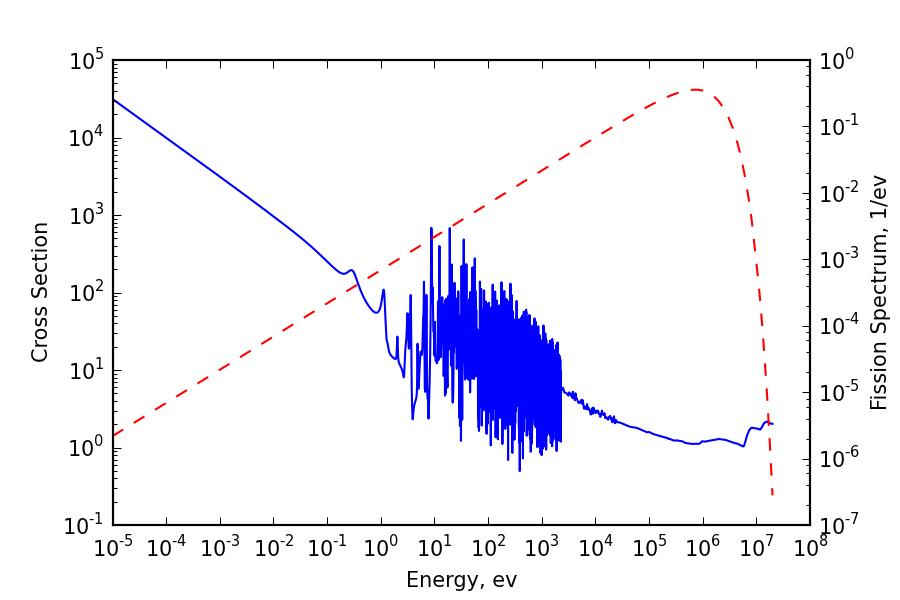
\includegraphics[width=0.75\textwidth]{u235fission.png}
  \caption{Fission cross section (blue) and fission spectrum (red) of uranium-235.}
  \label{fig::u235fission}
\end{figure}

These three energy ranges (fission spectrum, slowing down, and thermal) each impact the neutron spectrum, \(\phi(E)\), in qualitatively different ways.  We can roughly characterize the spectrum in each range by introducing some approximations that permit an analytical solution to the neutron balance equation.
\subsubsection{Fission Energy Range}
\label{sec:orgheadline29}
Neutrons are typically emitted from fission with a kinetic energy of 1 to 2 MeV.  This is much higher than the thermal equilibrium energy that is on the order of 1 eV.  At these high energies, the rate of neutrons being created in interval \(dE\) from fission is much greater than neutrons being scattered into \(dE\) from lower energies.  Thus
\begin{align}
  \phi(E) dE \approx  \frac{\chi(E)}{k_\infty\Sigma_t(E)} \int_0^\infty dE' \nu\Sigma_f(E') \phi(E')  dE = \frac{\chi(E)}{\Sigma_t(E)} \times \text{ constant}.
\end{align}
Thus the neutron spectrum at high energies, say \(E > 0.5 MeV\), is roughly proportional to the fission spectrum divided by the total cross section.

The fission spectrum can be described by a number of different formulations, one of which is the Watt spectrum.  The Watt spectrum is a probability density that can be written
\begin{align}
  p_\text{Watt}(E) = \frac{1}{I} \sinh\sqrt{bE} e^{-E/a}
\end{align}
where \(I\) is a normalization constant, and \(a\) and \(b\) are parameters.  For uranium-235,
\begin{align}
  I &= 2.0555, \\
  a &= 1, \\
  b &= 2,
\end{align}
for \(E\) in MeV.  Integrating this function reveals that roughly 88\% of neutrons are created with an energy between 0.1 and 4 MeV, and only 1.4\% are created with an energy \emph{less} than 0.1 MeV.  The average energy is 2 MeV and the median is about 1.6 MeV.

\subsubsection{Slowing-Down Energy Range}
\label{sec:orgheadline30}
At energies between 1 eV and 50 keV, there are very few neutrons created directly from fission and elastic scattering is much more important than inelastic scattering.  (Why?)  The elastic scattering cross kernel can be written
\begin{align}
  \Sigma_s(E' \rightarrow E) = 
  \begin{cases}
    \frac{\Sigma_s(E')}{E'(1-\alpha)}, & E \leq E' \leq \frac{E}{\alpha} \\
    0, & \text{otherwise}
  \end{cases}
\end{align}
where \(\alpha = \left[(A-1)/(A+1)\right]^2\).  If there are \(J\) nuclides present then the neutron balance equation becomes
\begin{align}
  \Sigma_t(E) \phi(E) dE
  = \sum_{j=1}^J \left[ \int_E^{E/\alpha_j} dE' \frac{\Sigma_s(E')}{E'(1-\alpha)} \phi(E') \right] dE.
\end{align}

Let's consider the case of neutron slowing down in the presence of hydrogen plus large resonance aborbers.  If the \(j=1\) nuclide is hydrogen (\(\alpha=0\)) and all the others are quite heavy (\(\alpha \approx 1\)) then we can write
\begin{align}
  \Sigma_t(E) \phi(E)
  &=  \left[ \int_E^\infty dE' \frac{\Sigma_s^H(E')}{E'} \phi(E') \right]
    + \sum_{j=2}^J \left[ \int_E^{E/\alpha_j} dE' \frac{\Sigma_s^j(E')}{E'(1-\alpha)} \phi(E') \right] \\
  &\approx  \int_E^\infty dE' \frac{\Sigma_s(E')}{E'} \phi(E')
    + \sum_{j=2}^J \frac{\Sigma_s(E)}{\alpha} \phi(E) 
\end{align}
where in the second approximation we have used \(\Sigma_s^j(E')\phi(E')/E' \approx \Sigma_s^j(E)\phi(E)/E\) for \(E' \in [E, E/\alpha_j]\).  This equation can be manipulated to yield (approximately
\begin{align}
  \left[ \Sigma_a(E) + \Sigma_s^H(E) \right] \phi(E)
  &= \int_E^\infty dE' \frac{\Sigma_s^H(E')}{E'} \phi(E')
\end{align}
where on the left-hand-side we have used \(\Sigma_s^H(E) \approx \Sigma_s(E) - \sum_{j=2}^J \Sigma_s^j(E)/\alpha\).  Differentiating this expression and defining a new function \(f(E) = \left[ \Sigma_a(E) + \Sigma_s^H(E) \right] \phi(E)\) leads to
\begin{align}
  \frac{df}{dE} &= - \frac{\Sigma_s^H(E)}{E\left[ \Sigma_a(E) + \Sigma_s^H(E) \right]} f(E).
\end{align}
This equation can be solved using an integrating factor and integrating from \(E\) to some arbitrary energy \(E_1\), ultimately leading to
\begin{align}
  \phi(E) = \frac{\left[ \Sigma_a(E_1) + \Sigma_s^H(E_1) \right] E_1 \phi(E_1)}{\left[ \Sigma_a(E) + \Sigma_s^H(E) \right] E}
            \exp\left[ -\int_E^{E_1} \frac{\Sigma_a(E')}{\left[ \Sigma_a(E') + \Sigma_s^H(E') \right] E'} dE' \right].
\end{align}
Thus \(\phi(E)\) varies fundamentally as \(1/E\) with localized perturbations caused by resonances that manifest in \(\Sigma_a(E)\) in the denominator of the first term and an overall attenuation arising from the exponential term, which again is primarily affected by resonances along the energy path from \(E_1\) to \(E\).

The fact that the flux will be locally depressed in the vicinity of a large absorption resonance is called \emph{energy self-shielding}.  The name suggests that because the neutron population is suppressed in a resonance energy range, the neutrons are naturally ``shielded'' from the resonance to some degree.

A rough estimate of the number of neutrons that will be absorbed by a given resonance can be obtained by approximating the number of neutrons that are attenuated by the resonance.  Assuming that within an absorption resonance of width \(\Delta E\) we will have \(\Sigma_a(E) >> \Sigma_s^H(E)\) leads to
\begin{align}
  \exp\left[ -\int_E^{E_1} \frac{\Sigma_a(E')}{\left[ \Sigma_a(E) + \Sigma_s^H(E) \right] E'} dE' \right]
  \approx \exp\left( -\int_E^{E+\Delta E} \frac{1}{E'} dE' \right)
  = \frac{1}{1+\Delta E/E}.
\end{align}
The first large resonance in uranium-238, for example is located at 6.67 eV with a width of about 0.027 eV.  Thus neutrons slowing down through the this resonance would be attenuated by a factor of roughly 0.996, which represents a loss of about 0.4\%.

\subsubsection{Thermal Energy Range}
\label{sec:orgheadline31}
We have previously noted that free atoms have random energies that obey the Maxwell-Boltzmann distribution, which written in terms of energy is
\begin{align}
  p_\text{MB}(E) = 2 \sqrt{\frac{E}{\pi}} \left( \frac{1}{kT} \right)^{3/2} \exp\left( - \frac{E}{kT} \right).
\end{align}
We might expect that as neutrons slow down to ``thermal'' energies they would assume the a similar energy profile, effectively becoming part of the equilibrium system.  This assumption would not be far off in general.

In fact, in the absence of absorption and a neutron source, the flux becomes
\begin{align}
  \label{eq::maxwellianFlux}
  \phi(E) = v(E) n_0 p_\text{MB}(E),
\end{align}
where \(v(E) = \sqrt{2E/m}\) and \(n_0\) is a normalization constant.  To show that this is so requires the \emph{principle of detailed balance}, which states that all scattering kernels possess the property
\begin{align}
  v(E') \Sigma_s(E' \rightarrow E) p_\text{MB}(E') = v(E) \Sigma_s(E \rightarrow E') p_\text{MB}(E).
\end{align}
Under the stated assumptions, the neutron balance equation becomes
\begin{align}
  \Sigma_s(E) \phi(E) = \int_0^\infty dE' \Sigma_s(E' \rightarrow E ) \phi(E').
\end{align}
Using the property of detailed balance and Eq. \eqref{eq::maxwellianFlux} in the above equation demonstrates that the Maxwellian flux given by Eq. \eqref{eq::maxwellianFlux} is indeed a solution.

Of course assuming that there is no source of neutrons, no absorption and no leakage is a stretch to say the least.  The effects of the slowing-down source, absorption and leakage tend to have the general effect of ``shifting'' the Maxwell-Boltzmann distribution up in temperature.  Thus one may replace \(T\) by some effective temperature, \(T_{\text{eff}}\), in \(p(E)\) to obtain a closer match to reality.

There are numerous sophisticated models for predicting the thermal neutron energy distributions, or one may simply solve the neutron balance equation numerically on a computer.  In either approach, an accurate model should include the effects of molecular and crystalline effects on nuclear motion (when they exist), as these are important factors at thermal energies.
\subsection{Elastically Scattering Through Energy}
\label{sec:orgheadline36}
In the section ``Neutron-Nucleus Reactions'' we observed that the fact that for a stationary target a neutron can be scattered from an energy \(E\) to an energy \(E' \in [\alpha E, E]\) where \(\alpha = (A-1)^2/(A+1)^2\).  In the following we will derive two quantities that will be useful in discussions resonance absorption: the average energy loss and the average lethargy loss in elastic collisions.  To derive the quantities we need the probability density function for scattering from \(E\) to \(E'\), which we will call \(P(E' \rightarrow E)\).

\subsubsection{Elastic Scattering Energy Change}
\label{sec:orgheadline33}
If we assume a stationary target we know that
\begin{align}
  \label{eq::elasticEnergyChange}
  \frac{E'}{E} = \frac{(1-\alpha) + (1-\alpha) \cos\phi}{2}
\end{align}
where \(\phi\) is the scattering deflection angle in the CM.  Thus energy change is correlated to the angle \(\phi\).  If scattering is isotropic in CM, then the probability of scattering through deflection angle \(\phi\) is
\begin{align}
  P(\phi) = \frac{1}{2}\sin\phi.
\end{align}
Because an incremental energy change \(dE'\) is correlated to a incremental scattering angle \(-d\phi\), we have
\begin{align}
  P(E \rightarrow E') dE = -P(\phi) d\phi.
\end{align}
Substituting the derivative of Eq. \eqref{eq::elasticEnergyChange} into this equation leads to
\begin{align}
  P(E \rightarrow E') = \frac{1}{E(1-\alpha)}.
\end{align}

\subsubsection{Average Energy Loss}
\label{sec:orgheadline34}
The average amount of energy lost in a scattering collision is given by
\begin{align}
  \left< \Delta E \right> = E - \int_{\alpha E}^E E' P(E \rightarrow E') dE' = \frac{1}{2}(1-\alpha)E.
\end{align}
Thus the average amount of energy lost per collision is proportional to the pre-collision energy and the mass term \(\alpha\).

\subsubsection{Average Logarithmic Energy Loss}
\label{sec:orgheadline35}
The average logarithmic energy loss per elastic collision (or equivalent, the average lethargy loss) is given by
\begin{align}
  \xi = \int_{\alpha E}^E \ln\left(\frac{E}{E'}\right) P(E \rightarrow E') dE' = 1 + \frac{\alpha}{1-\alpha} \ln\alpha.
\end{align}
Note that hydrogen, \(\alpha = 0\) and the equation can not evaluated directly, but it can be shown that \(\lim_{\alpha \rightarrow 0} \xi = 1\).  Also note that this value is independent of \(E\).

\subsection{Resonance Absorption}
\label{sec:orgheadline40}
To calculate a local neutron spectrum (independent of space) one could solve the slowing-down equation numerically to an arbitrary degree of accuracy.  An analytically exact solution is generally not possible due to the complex dependence of the cross section on energy, including many closely-spaced and unresolved resonances.  If we consider a very simplistic case, however, we can make some reasonable approximations that lead to closed-form expressions of the flux spectrum.  These approximation are rarely used in production-level software anymore, but they permit insight that is generally not available from purely numerical solutions.  

Assume that a medium consists of a single moderating material whose scattering cross sections is much larger than its absorption cross section (\(\Sigma_s^M >> \Sigma_a^M\)) and a resonance isotope.  We will consider the problem of estimating the neutron flux inside of a \emph{single} resonance within the resonance isotope.  The neutron balance equation in this case can be written
\begin{align}
  \left[ \Sigma_t^\text{res}(E) + \Sigma_s^M(E) \right] \phi(E)
  = \int_E^{E/\alpha_M} \frac{\Sigma_s^M(E') \phi(E')}{E'(1-\alpha_M)} dE'
  + \int_E^{E/\alpha_\text{res}} \frac{\Sigma_s^\text{res}(E') \phi(E')}{E'(1-\alpha_\text{res})} dE',
\end{align}
where we have also assumed that \(\Sigma_s^M\) is roughly constant over the energy range of interest.  In fact we may assume that the moderator scattering cross section is roughly equal to the potential cross section of the moderating isotope.

It was previously observed that the neutron flux tends to vary as \(1/E\) in the resonance range.  This variation of the flux is asymptotically valid, away from resonances peaks.  If we normalize the flux so that \(\phi(E) = 1/E\) above the resonance currently in question, then substitute this value into the first integral in the balance equation we have
\begin{align}
  \left[ \Sigma_t^\text{res}(E) + \Sigma_s^M \right] \phi(E)
  = \frac{\Sigma_s^M}{E} +
    \int_E^{E/\alpha_\text{res}} \frac{\Sigma_s^\text{res}(E') \phi(E')}{E'(1-\alpha_\text{res})} dE'.
\end{align}

For the sake of simplicity, we will consider only a single resonance that is well-separated from other resonances, in which case the SLBW formula is applicable.  The \emph{practical width} of a resonance is a heuristic measurement for the ``reach'' of a given resonance in terms of energy.  This practical width can be formed by comparing the \emph{potential} cross section, \(\sigma_p^\ell\), with \(\sigma_0\) in the SLBW capture cross section.  Looking for an effective width that produces \(\sigma_0/\sigma_p^0 \approx 1\) leads to the practical width
\begin{align}
  \Gamma_p \approx \sqrt{\frac{\sigma_0}{\sigma_p^0}} \Gamma_{x,i}.
\end{align}
In general the practical width \(\Gamma_p\) will be larger than the actual width \(\Gamma_{x,i}\).  We will use the practical width only as a rule of thumb in determining how narrow (or wide) a resonance effectively is.

\subsubsection{Narrow Resonance Approximation}
\label{sec:orgheadline37}
If the practical width of a resonance is much smaller than the average energy loss due to elastic scattering (i.e., \(\Gamma_p << E_i(1-\alpha_M)/2\)), then it is likely that a neutron will ``jump over'' the resonance.  Thus, as we did with the moderating integral, we may assume that the flux takes it's asymptotic \(1/E\) shape in the resonance integral.  We may also assume that the \(\Sigma_s^\text{res} \approx \Sigma_p^{0,\text{res}}\), which is independent of energy for \(a / \lambda << 1\).  This leads to
\begin{align}
  \left[ \Sigma_t^\text{res}(E) + \Sigma_s^M \right] \phi(E)
  = \frac{\Sigma_s^M}{E}
  + \frac{\Sigma_p^{0,\text{res}}}{E}.
\end{align}
This is called the \emph{narrow resonance approximation} and produces the flux
\begin{align}
  \phi_\text{NR}(E)
  = \frac{\Sigma_s^M + \Sigma_p^{0,\text{res}}}{\left[ \Sigma_t^\text{res}(E) + \Sigma_s^M \right]E}.
\end{align}

\subsubsection{Wide Resonance Approximation}
\label{sec:orgheadline38}
If the practical width of a resonance is large compared with the average energy loss due to elastic scattering (i.e., \(\Gamma_p >> E_i(1-\alpha_M)/2\)), then it is likely that a neutron will experience a reaction inside the resonance peak.  In this case we will not assume the flux has it's asymptotic form, but rather that \(\frac{\Sigma_s^\text{res}(E') \phi(E')}{E')} \approx \frac{\Sigma_s^\text{res}(E) \phi(E)}{E)}\) within the in-scattering range of the resonance material, which is small because \(\alpha_\text{res} \approx 1\).  This leads to
\begin{align}
  \phi_\text{WR}(E)
  = \frac{\Sigma_s^M}{\left[ \Sigma_a^\text{res}(E) + \Sigma_s^M \right] E}.
\end{align}
This is known as the \emph{wide resonance approximation} (which emphasizes the relationship between the practical resonance width and the average energy loss) or the \emph{narrow resonance, infinite mass approximation} (which emphasizes the assumption that \(\alpha_\text{res} \approx 1\)).

\subsubsection{Resonance Integral}
\label{sec:orgheadline39}
Once the spectrum \(\phi(E)\) has been determined, we may use it to evaluate the total absorption rate due to the resonance.  This information is normally computed as the \emph{resonance integral},
\begin{align}
  I_{\gamma,i} = \frac{R_{\gamma,i}}{N^\text{res}} = \int_0^\infty \sigma_{\gamma,i}(E) \phi(E) dE.
\end{align}
The resonance integral is useful for calculating the \emph{resonance escape probability} and multigroup cross sections, which we will discuss later.
\subsection{Problems}
\label{sec:orgheadline41}
\begin{enumerate}
\item Derive the the solution \(\phi(E)\) using the narrow and wide resonance approximations.
\end{enumerate}
\subsection{References}
\label{sec:orgheadline42}
\begin{itemize}
\item Stacey
\item Duderstadt and Hamilton
\end{itemize}
\section{Neutron Transport}
\label{sec:orgheadline57}
At this point we have characterized neutron-nucleus interactions and described the physics of a neutron slowing down from high (fission) energies to low (thermal) energies in the presence of moderators and resonance absorbers.  We will now proceed to a full description of neutron transport, the goal of which is to describe how neutrons are distributed through space and energy as a function of time.

\subsection{Fundamental Concepts and Variables}
\label{sec:orgheadline47}
We know that a scattering reaction will tend to change the kinetic energy of a neutron and the direction in which it is traveling.  Thus our attempt to describe the distribution of neutrons must take into account space (where neutrons are), energy (how fast they are moving), angle (in what direction they are moving) and time.  This collection of independent variables is called the \emph{phase space} of neutron transport.

The space parameter will be denoted by the variable \(\vec{r}\).  While it is possible to represent this vector in any number coordinate systems, we will focus on Cartesian systems so that space can be represented by vectors of the form \(\vec{r} = x\vec{i} + y\vec{j} + z \vec{k}\).  In three-dimensional (Cartesian) space the differential space element is a differential volume \(dV = dx dy dz\).

A neutrons direction (or angle) at a given point is given by the unit vector \(\vec{\Omega}\).  The definition and properties of \(\vec{\Omega}\) is given in the ``Mathematical Odds and Ends'' appendix accompanying these notes.  The angle \(\vec{\Omega}\) can be described in terms of its projections along each of three Cartesian coordinate axes, \(\vec{\Omega} = \Omega_x \vec{i} + \Omega_y \vec{j} + \Omega_z \vec{k}\), or in terms of the polar and azimuthal angles \(\theta\) and \(\varphi\), \(\vec{\Omega} = \sin\theta \cos\varphi \vec{i} + \sin\theta \sin\varphi \vec{j} + \cos\theta \vec{k}\).  In three dimensions the differential \emph{solid angle} is \(d\vec{\Omega} = \sin\theta d\varphi d\theta\).

\subsubsection{Neutron Density}
\label{sec:orgheadline44}
Because there is such a high density of neutrons in a reactor and their collisions are probabilistic, it is infeasible to determine the location and velocity of every single neutron, nor would such an abundance of information be particularly useful.  Instead we will attempt to determine the \emph{expected} number of a neutrons within differential space, angle and energy elements as a function of time:
\begin{align}
  n(\vec{r},\vec{\Omega},E,t) dV d\vec{\Omega} dt.
\end{align}
The function \(n(\vec{r},\vec{\Omega},E,t)\) in this quantity is the \emph{neutron angular density}.  We may also define the \emph{neutron scalar density} as the expected number of neutrons in all directions, \(n(\vec{r},E,t) = \int_{4\pi} n(\vec{r},\vec{\Omega},E,t) d\vec{\Omega}\).

\subsubsection{Neutron Flux}
\label{sec:orgheadline45}
We know that the reaction rate density (i.e., the number of neutron interactions per unit volume per unit time) is the product of the nuclelar density, the microscopic cross section for the reaction, the neutron speed and the neutron density.  The product of the first two parameters is called the macroscopic cross section, while the product of the latter two parameters is called the neutron flux.  If we write the neutron flux to explicitly include variation with respect to angle then we have the \emph{angular neutron flux}, \(\psi(\vec{r},\vec{\Omega},E,t) = v(E)n(\vec{r},\vec{\Omega},E,t)\).  If we integrate over all angles then we have the \emph{scalar neutron flux}, \(\phi(\vec{r},E,t) = \int_{4\pi} \psi(\vec{r},\vec{\Omega},E,t)\).

Knowing the angular and scalar fluxes is valuable because it enables us to compute reaction rates, including the rate at which energy is produced from fission reactions.  An intuitive interpretation of these functions, however, is not immediately evident.  Recall that the neutron \emph{speed} is the differential path length divided by a differential unit of time.  The product of the neutron density with speed (i.e., flux) is therefore the \emph{total path length} traversed by all neutrons per unit volume per unit time.  Thus multiplying flux by the macroscopic cross section (probability of interaction per unit path length) gives us interactions per unit volume per unit time.  The \emph{angular} flux is the total path length of all the neutrons moving along a given direction; the \emph{scalar} flux is the total path length of all the neutrons regardless of direction.

\subsubsection{Neutron Current}
\label{sec:orgheadline46}
If we multiply the angular neutron density by the vector velocity then we get the \emph{angular neutron current}: \(\vec{J}(\vec{r},\vec{\Omega},E,t) = \vec{v}(\vec{\Omega},E) n(\vec{r},\vec{\Omega},E,t)\).  Integrating this variable over all angles provides a vector-valued quantity which is usually just called \emph{neutron current}: \(\vec{J}(\vec{r},E,t) = \int_{4\pi} \vec{v}(\vec{\Omega},E) n(\vec{r},\vec{\Omega},E,t) d\vec{\Omega}\).  Noting \(\vec{v}(\vec{\Omega},E) = \vec{\Omega}v(E)\) permits writing the current in terms of the angular neutron flux.

The neutron current is a useful quantity because it allows us to calculate the net rate at which neutrons are ``flowing'' through a surface.  In particular, the rate at which neutrons with energy \(E\) are crossing a differential surface with area \(dA\) and unit normal vector \(\vec{n}\) is given by
\begin{align}
  dA \left( \vec{n} \cdot \vec{J}(\vec{r},E,t) \right).
\end{align}

Occasionally it is useful to represent the total number of neutrons passing in to or out from a system through a surface.  At a point, these quantities are called the partial currents.  The incoming and outgoing partial currents can be expressed as follows:
\begin{align}
  j^+(\vec{r},E,t) &= \int_{\vec{n}\cdot\vec{\Omega}>0} \vec{n} \cdot \vec{\Omega} \psi(\vec{r},E,t) d\vec{\Omega} \rightarrow \text{outgoing partial current},s \\
  j^-(\vec{r},E,t) &= -\int_{\vec{n}\cdot\vec{\Omega}<0} \vec{n} \cdot \vec{\Omega} \psi(\vec{r},E,t) d\vec{\Omega} \rightarrow \text{incoming partial current}.
\end{align}
Note that the \emph{net} number of neutrons passing through this surface (per unit area) then becomes \(j^+ - j^- = \vec{n}\cdot\vec{J}\).

\begin{table}
  \centering
  \caption{Basic quantities in neutron transport}
  \begin{tabular}{ll}
  \hline
  Angular density & $n(\vec{r},\vec{\Omega},E,t)$ \\
  Angular flux & $\psi(\vec{r},\vec{\Omega},E,t) = v(E) n(\vec{r},\vec{\Omega},E,t)$ \\
  Scalar flux & $\phi(\vec{r},E,t) = \int_{4\pi} \psi(\vec{r},\vec{\Omega},E,t) d\vec{\Omega}$ \\
  Current & $\vec{J}(\vec{r},E,t) = \int_{4\pi} \vec{\Omega} \psi(\vec{r},\vec{\Omega},E,t)$ \\
  \hline
  \end{tabular}
\end{table}

\subsection{The Transport Equation}
\label{sec:orgheadline53}
A transport equation for neutrons can be obtained by performing a neutron balance about an element \(dV d\vec{\Omega} dE dt\) in phase space.  We make the following assumptions
\begin{enumerate}
\item Neutrons travel in straight line between collisions.
\item Neutron exists as points in space, with negligible size.
\item Neutron-neutron interactions can be neglected.
\item Neutron-nucleus interactions occur instantaneously.
\item The material is isotropic.
\item When scattering, the deflection of a neutron's trajectory from \(\vec{\Omega}'\) to \(\vec{\Omega}\) is a function of the cosine of the angle between the original and final unit directions, i.e. \(\vec{\Omega}' \cdot \vec{\Omega}\).
\end{enumerate}

We will make several additional assumptions at this point that, while not necessary, are very accurate and lead to a simpler form of the transport equation.
\begin{enumerate}
\item Fission neutrons are emitted isotropically in the LAB.
\item The average number fission neutrons is independent of the energy of the neutron that caused the fission.
\item The only reaction that generates neutrons if fission.
\end{enumerate}
In reality, assumptions 2 and 3 will lead to small errors in the transport solution, but typically the cross sections to account for these effects implicitly.  Specifically the quantity \(\nu\Sigma_f(E)\) is usually treated as a single quantity so that the energy variation of \(\nu\) is embedded in \(\Sigma_f(E)\).  With regards to assumption 3, some highly excited heavy nuclei may exist two or three neutrons, leading to (n,2n) or (n,3n) reactions.  The additional neutrons in this case can be accounted for by normalizing the overall scattering to the average number of neutrons emitted, which will be very close to one.

The final form of the transport equation given these assumptions is
\begin{align}
  \frac{1}{v} \frac{\partial\psi}{\partial t}
  + \vec{\Omega} \cdot \nabla\psi
  + \Sigma \psi
  &= \int_0^\infty dE' \int_{4\pi} \Sigma_s(\vec{r},E' \rightarrow E, \vec{\Omega}'\cdot\vec{\Omega}) \psi(\vec{r},\vec{\Omega}',E',t) \notag\\
  &+ \frac{\chi(E)}{4\pi} \int_0^\infty dE' \int_{4\pi} \nu\Sigma_f(\vec{r},E') \psi(\vec{r},\vec{\Omega}',E',t)
  + q_\text{ext}(\vec{r},\vec{\Omega},E,t).
  \label{eq::transportEqn}
\end{align}
For completeness, consider the transport equation to be solved for a region \(V\) so that \(\vec{r} \in V\).  We will also take \(E \in [0, \infty]\), although in practice a maximum and minimum energy are adopted so that the flux is negligible outside of the that interval.

As with any mathematical model, we must consider under what conditions our transport equation has a viable solution.  To answer this question rigorously one should turn to the tools and theory of mathematics.  Arguments based on physics intuition, however, will lead largely to the same conclusions given sufficient clarity of thought.  We will therefore focus on intuitive arguments.

\subsubsection{Boundary Conditions}
\label{sec:orgheadline48}
As with any differential equation, we must supply appropriate boundary conditions.  Let us presently denote the boundary of \(V\) by \(\partial V\).  When solving the neutron transport equation for the angular flux, the boundary condition specifies the number of neutrons \emph{entering} the system.  There are several ways to provide this boundary source.  The simplest is the \emph{fixed flux} boundary condition, which has the following form:
\begin{align}
  \psi(\vec{r},\vec{\Omega},E,t) = \psi_\text{inc}(\vec{r},\vec{\Omega},E,t)
\end{align}
where \(\psi_\text{inc}\) is given a function for \(\vec{r} \in \partial V\) and \(\vec{\Omega} \cdot \vec{n} < 0\) with \(\vec{n}\) the outward unit normal vector on the surface \(\partial V\).  If \(\psi_\text{inc} = 0\) then we have the \emph{vacuum} condition, which means that there are no incoming neutrons.

Most reactors exhibit a high degree of spatial repetition, fuel rods in an assembly lattice being the prime example.  A common approximation in modeling a single fuel rod is to assume that the lattice repeats infinitely in the radial directions.  Thus each fuel rod looks like every other fuel rod.  This form of symmetry can be exploited by placing mirror boundary conditions known as \emph{specular reflection} between the rods.  In this type of reflection we have
\begin{align}
  \psi(\vec{r},\vec{\Omega},E,t) = \psi(\vec{r},\vec{\Omega}',E,t)
\end{align}
where \(\vec{\Omega}\) is the incoming direction corresponding to mirror reflection of \(\vec{\Omega}'\) outgoing direction.  Mathematically this means \(\vec{\Omega} \cdot \vec{n} = - \vec{\Omega}' \cdot \vec{n}\) and \(\left(\vec{\Omega} \times \vec{\Omega}'\right) \cdot \vec{n} = 0\).

Vaccum and specular reflection boundary conditions are by far the most common.  Other possible boundary conditions are \emph{white reflection}, in which outgoing neutrons are distributed uniformly across all incoming directions, and periodic boundary conditions, which account for translational and rotational symmetry.

\subsubsection{Initial Condition}
\label{sec:orgheadline49}
Because the transport equation, as it is written, is time-dependent, we must also supply an initial condition.  The initial condition is simply
\begin{align}
  \psi(\vec{r},\vec{\Omega},E,0) = \psi_0(\vec{r},\vec{\Omega},E)
\end{align}
with \(\psi_0\) a given function for \(\vec{r} \in V\).

\subsubsection{Existence of a Steady-State Solution}
\label{sec:orgheadline50}
We often want to determine the ``steady-state'' flux solution for a system that is in some form of equilibrium.  In general, Eq. \eqref{eq::transportEqn} may or may not have a steady-state solution.  The complicating factor is fission.  If more neutrons are begin created from fission than lost by all capture and leakage, then the chain reaction will drive the neutron population perpetually upward.  If the opposite is true then the neutron population will rapidly decrease.  Thus steady-state is only obtained when there is a \emph{precise} balance between production and loss.  

If neutron loss (by leakage or capture) is much more likely than neutron production by fission (called a sub-critical configuration), then we will have a steady-state solution as long as the external source term, \(q\) is non-zero.  These problems are called \emph{fixed-source} problems, and include accelerator systems, radiation shielding, and sub-critical reactors as a characteristic examples.  If \(q=0\) then there will be only the trivial solution.

In reactor design and analysis, however, we frequently want to determine the steady-state power distribution corresponding to a ``critical reactor'' in which neutron production is exactly balanced by neutron loss.  In this case the external source of neutrons, \(q(\vec{r},\vec{\Omega},E,t)\), is either zero or negligible, and the transport equation becomes
\begin{align}
  \vec{\Omega} \cdot \nabla\psi(\vec{r},\vec{\Omega},E)
  + \Sigma(\vec{r},\vec{\Omega}) \psi(\vec{r},\vec{\Omega},E)
  &= \int_0^\infty dE' \int_{4\pi} \Sigma(\vec{r},E' \rightarrow E, \vec{\Omega}'\cdot\vec{\Omega}) \psi(\vec{r},\vec{\Omega}',E') \notag\\
  &+ \frac{\chi(E)}{4\pi} \int_0^\infty dE' \int_{4\pi} \nu\Sigma_f(\vec{r},E') \psi(\vec{r},\vec{\Omega}',E').
  \label{eq::ssTransportEqn}
\end{align}
As it is written, Eq. \eqref{eq::ssTransportEqn} will practically \emph{never} have a solution.  Any imbalance in the transport equation, whether due to the physical configuration, cross section uncertainties, or numerical error, will cause the equation to be unsolvable because no corresponding steady-state solution exists.  Solvability exists at the infinitesimal point where all of the cross section values align to produce a precisely balanced system.  Numerically there is no hope in finding this magical point.

We may not be able to model the reactor precisely enough to determine a steady-state solution, but we can look for a solution that is ``close'' to a steady-state solution.  This is accomplished by introducing a scaling factor, typically on the fission term.  Calling this scaling factor \(\lambda\) the transport equation becomes
\begin{align}
  \vec{\Omega} \cdot \nabla\psi(\vec{r},\vec{\Omega},E)
  + \Sigma(\vec{r},E) \psi(\vec{r},\vec{\Omega},E)
  &= \int_0^\infty dE' \int_{4\pi} \Sigma_s(\vec{r},E' \rightarrow E, \vec{\Omega}'\cdot\vec{\Omega}) \psi(\vec{r},\vec{\Omega}',E') \notag\\
  &+ \lambda\frac{\chi(E)}{4\pi} \int_0^\infty dE' \int_{4\pi} \nu\Sigma_f(\vec{r},E') \psi(\vec{r},\vec{\Omega}',E').
  \label{eq::eigTransportEqn}
\end{align}
The factor \(\lambda\) adds a ``knob'' so that we can dial-in a solution that approximates the reactor's steady-state, given that our naive numerical model has no chance of being precise enough.  The closer \(\lambda\) is to one, the closer we are to a legitimate steady-state solution.  It is common to call the inverse of \(\lambda\) the \emph{effective multiplication factor}, or \(k_\text{eff} = \lambda^{-1}\), because it represents the rate at which the neutron population would be increasing (or multiplying) if this system were ``real.''  Inspection of Eq. \eqref{eq::eigTransportEqn} reveals that it is in fact a generalized eigenvalue problem with \(\lambda\) the eigenvalue.  The equation may be massaged into a traditional eigenvalue problem with \(k_\text{eff}\) the eigenvalue.  We will discuss this further at a later time.

A final practical consideration is that the eigenvalue form of the transport equation is homogeneous and linear in the angular flux.  This means that the angular flux can be arbitrarily scaled and the solution remains valid.  (This is the typical behavior of eigenvalue problems.)  Thus to determine a \emph{unique} solution, we must provide an additional constraint.  Typically the total reactor power fulfills this requirement.

\subsubsection{What just happened?}
\label{sec:orgheadline51}
It is very easy at this point to be temporarily blinded by the sudden onslaught of mathematical technicality that has attacked our transport equation.  It is worth a moments time to consider what happens in a real reactor so that we remain somewhat oriented with respect to reality.  If you have not been previously exposed to reactor physics or reactor operations (or have not paid attention to such discussions) then some of the following must be taken initially on faith.

First, in the previous section we painted a very bleak picture of a steady-state reactor being balanced on a precipice between explosion and stagnation.  Commercial reactors, however, are designed to inherently be quite stable beasts.  One of the most important stabilizing factors has already been introduced in these notes, which is the Doppler broadening of capture cross sections.  If a reactor is generating more neutrons from fission than are being lost, then the neutron population will increase and the fission reaction rate will follow in lock-step.  As power increases temperature will rise.  You have seen that increasing the temperature of an isotope with capture resonance will increase the capture rate of neutrons.  This increase in capture rate will naturally arrest a modest increase in power and bring the system into steady-state at a naturally-attained equilibrium temperature.  The same sequence will happen in the opposite direction for a decreasing neutron population.  A second stabilizing effect occurs when, as in the case of modern commercial reactors, the coolant serves double-duty as the moderator.  As temperature increases, the moderator density decreases, often leading decrease in the thermalization of neutrons.

We now see that obtaining a ``real'' steady-state solution would require solving not just the transport equation, but heat transfer and likely fluid dynamics equations as well.  Moreover introducing temperature (and density) as variables leads to nonlinearities in the transport equation.  In short, the not-so-simple transport equation just become orders of magnitude more challenging to solve.  So instead, how about we hold temperature constant (say at an average value), then solve the transport equation approximately by scaling fission to account for the fact that we are neglecting stabilizing feedback mechanisms.  The eigenvalue approach should look quite appealing at this point!

\subsubsection{Solving the Transport Equation}
\label{sec:orgheadline52}
Finding a closed-form solution of the transport equation is impossible for all but the simplest of cases.  In practice we must adopt both physical and numerical approximations.  Following is a partial list of complications we should expect.
\begin{enumerate}
\item Most mathematical theory deals with either partial differential equations \emph{or} integral equations.  The transport equation is an \emph{integro-differential} equation containing both an integral and gradient term.
\item The dimensionality of the phase space is quite high.  Three dimensions in space, two in angle, one in energy and one in time leads to a seven-dimensional space in the most general setting.  Numerically this will generate a very large number of unknowns that must be solved.
\item The energy dependence of the cross sections is very complex because of resonances.  Representing these cross sections numerically a very large number of discretization points.
\item The size of virtually all reactors is much greater than the neutron mean-free-path.  Thus any spatial discretization must include a large number of points.
\end{enumerate}

On the other hand, the transport equation is linear, so if we can manage the \emph{size} of the problem then we shouldn't loose too much sleep.  Given advances in modern computing, we are able to calculate much larger and more accurate transport solutions than ever before.  Nevertheless, solving large transport problems is very challenging.  Our goal presently is not to explore the computational approaches to this problem in any significant detail, but rather present an overview of the approximations and strategies that are made to solve neutron transport for reactor physics analyses.

\subsection{The Multigroup Approximation}
\label{sec:orgheadline54}
In the previous section we examined the behavior of neutrons with respect to the energy variable.  The neutron balance equation we derived there was actually the transport equation for an infinitely large, homogeneous region.  Under those conditions, \(\nabla\psi = \vec{0}\), and the flux did not depend on angle because of rotational symmetry.  We will now introduce an approximation that will lead to a simpler energy landscape so that we can devote more attention to spatial variations of the neutron flux.

The \emph{multigroup approximation} attempts to simplify the energy-dependent description of neutron transport by binning neutrons to ``groups'' based on their energy.  To begin, pick a set of energy group boundaries, 
\begin{align}
  E_G < E_{G-1} < E_{G-2} < \hdots < E_g < \hdots < E_2 < E_1 < E_0.
\end{align}
Note that (for historical reasons) \(E_0\) is the highest energy, while \(E_G\) is the lowest energy.  Energy group \(g\) is defined by the interval \([E_g, E_{g-1}]\).  

Next, integrate the transport equation over a single energy group.  We may use any of variant of the transport equation.  Going with the eigenvalue form [Eq. \eqref{eq::eigTransportEqn}] produces an equation that can be written
\begin{align}
  \vec{\Omega} \cdot \nabla \psi_g(\vec{r},\vec{\Omega})
  + \Sigma_g(\vec{r}) \psi_g(\vec{r},\vec{\Omega})
  &= \sum_{g'=1}^G \int_{4\pi} \Sigma_{g'\rightarrow g}(\vec{r}, \vec{\Omega}'\cdot\vec{\Omega}) \psi_g'(\vec{r},\vec{\Omega}') d\vec{\Omega}' \notag\\
  &+ \lambda\frac{\chi_g}{4\pi} \sum_{g'=1}^G \int_{4\pi} \nu\Sigma_{f,g'}(\vec{r}) \psi_g'(\vec{r},\vec{\Omega}') d\vec{\Omega}'.
  \label{eq::mgTransportEqn}
\end{align}
where we have defined
\begin{align}
  \psi_g(\vec{r},\vec{\Omega}) &= \int_{E_g}^{E_g} dE \psi(\vec{r},\vec{\Omega},E), \\
  \Sigma_g(\vec{r}) &= \frac{\int_{E_g}^{E_g} dE \Sigma(\vec{r},E) \psi(\vec{r},\vec{\Omega},E)}{\int_{E_g}^{E_g} dE \psi(\vec{r},\vec{\Omega},E)}, \\
  \nu\Sigma_{f,g}(\vec{r}) &= \frac{\int_{E_g}^{E_g} dE \nu\Sigma_f(\vec{r},E) \psi(\vec{r},\vec{\Omega},E)}{\int_{E_g}^{E_g} dE \psi(\vec{r},\vec{\Omega},E)}, \\
  \chi_g &=  \int_{E_g}^{E_g} dE \chi(E), \\
  \Sigma_{g'\rightarrow g}(\vec{r}, \vec{\Omega}'\cdot\vec{\Omega} &= 
    \frac{\int_{E_g}^{E_g} dE \int_{E_{g'}}^{E_{g'}} dE' \Sigma_s(\vec{r},E' \rightarrow E, \vec{\Omega}'\cdot\vec{\Omega}) \psi(\vec{r},\vec{\Omega},E)}{\int_{E_g}^{E_g} dE \psi(\vec{r},\vec{\Omega},E)}.
\end{align}
The above parameters are called the multigroup constants and Eq. \eqref{eq::mgTransportEqn} the multigroup transport equation.  

The benefit of the multigroup equation is that \emph{if} we can calculate the multigroup constants, we can obtain a flux solution by solving the \(G\) coupled group equations for \(\psi_g\) rather than the transport equation that depends continuously on energy.  If \(G\) is chosen to be smaller than the number of points required to represent the most complex cross section (which is often in thousands), then we have simplified the computational task of solving the transport equation.  In practice, \(G\) may be be as large as a few hundred to as few as two.

Of course there is a catch-22 in that we need the detailed flux spectrum, \(\psi(\vec{r},\vec{\Omega},E)\), to calculate the group constants, but if we had the detailed flux spectrum then we could immediately calculate the group fluxes!  This is where an approximation is leveraged to maximize accuracy in the energy variable at the expense of the spatial variable.  Because most reactors feature regular arrays of fuel rods, symmetry can be used to simplify the transport problem.  Often a reactor physics calculations begins by solving the transport equation with 100's or 1000's of energy grid points in an infinite medium (0D), infinitely tall cylinder (1D) or occasionally a square pin-cell (2D).  Reflective boundary conditions around the simplified problem introduce an approximation, but if the neutron spectrum changes slowly with respect to space then the approximation is reasonable because the spectrum is only used as a weighting function to generate the multigroup cross sections.  In the past when computing power was scarce, the spectrum was obtained not by solving the transport equation, but simply by gluing a fission spectrum, a \(1/E\) intermediate spectrum and a thermal spectrum together.

Once an appropriate spectrum has been used to generate the multigroup constants, one may attempt to solve the transport equation for more complex geometries because the burden of excessive energy complexity has been lightened.  A single assembly calculation may use tens to a few hundred energy groups; a full-core calculation may use as few as two energy groups.

\subsection{Numerical Solutions of the Mutligroup Equation}
\label{sec:orgheadline56}
The multigroup approximation effectively handles the energy dependence of the transport equation (given a suitably accurate weighting spectrum for the cross section collapsing.)  There are several ways to discretize the equation with respect to angle.  In what follows we will look at the spherical harmonics (or \(P_N\)) and discrete ordinates (or \(S_N\)) approaches.  For simplicity our discussion will be limited to one spatial dimension.  Adopting the \(z\) direction (aligned with the \(\vec{k}\) unit direction) as the dimension of choice, the multigroup transport equation becomes
\begin{align}
  \mu \frac{\partial \psi_g(z,\mu)}{\partial z}
  + \Sigma_g(z) \psi_g(z,\mu)
  &= \sum_{g'=1}^G \int_{-1}^1 \Sigma_{g'\rightarrow g}(z, \mu_0) \psi_g'(z,\mu') d\mu' \\
  &+ \lambda\frac{\chi_g}{2} \sum_{g'=1}^G \int_{-1}^1 \nu\Sigma_{f,g'}(z) \psi_g'(z,\mu') d\mu'.
  \label{eq::1dMgTransportEqn}
\end{align}
Note that in obtaining this equation we have set \(\frac{\partial \psi}{\partial x} = \frac{\partial \psi}{\partial y} = 0\), integrated over all azimuthal angles, and set \(\mu=\cos\theta\) where \(\theta \in [0,\pi]\) is the polar angle.  We have additionally defined \(\mu_0 = \vec{\Omega}\cdot\vec{\Omega}' = \cos\theta_0\) as the cosine of the scattering deflection angle.

Before presenting the angular treatment of the transport equation, let's first consider a practical treatment of of the scattering cross section angular dependence.  As discussed in the appendix, the Legendre polynomials provide a basis for representing functions defined on the interval \([-1,1]\).  Because \(\theta_0 \in [0,\pi]\), the scattering cross section is just such a function when the position and group indices are fixed.  Specifically, let
\begin{align}
  \Sigma_{g'\rightarrow g}(z, \mu_0) = \sum_{\ell=0}^\infty \frac{2\ell+1}{2} \Sigma_{g' \rightarrow g}^\ell(z) P_\ell(\mu_0)
\end{align}
where \(P_\ell(\mu_0)\) is the \(\ell^\text{th}\) Legendre polynomial.  Multiplying this equation by \(P_{\ell'}(\mu_0)\), integrating over \(\mu_0\), and applying the orthogonality relationship leads to
\begin{align}
  \Sigma_{g' \rightarrow g}^\ell(z) = \int_{-1}^1 P_{\ell}(\mu_0)\Sigma_{g'\rightarrow g}(z, \mu_0) d\mu_0.
\end{align}
The \(\Sigma_{g' \rightarrow g}^\ell(z)\) coefficients are called the scattering moments.

Inserting the scattering kernel expansion into the transport equation provides
\begin{align}
  \mu \frac{\partial \psi_g(z,\mu)}{\partial z}
  + \Sigma_g(z) \psi_g(z,\mu)
  &= \sum_{g'=1}^G \sum_{\ell=0}^\infty \frac{2\ell+1}{2} \int_{-1}^1 \Sigma_{g' \rightarrow g}^\ell(z) P_\ell(\mu_0) \psi_g'(z,\mu') d\mu' \\
  &+ \lambda\frac{\chi_g}{2} \sum_{g'=1}^G \int_{-1}^1 \nu\Sigma_{f,g'}(z) \psi_g'(z,\mu') d\mu'.
\end{align}
Using the addition theorem of Legendre polynomials allows us to write the polynomial \(\mu_0\) as the product of polynomials in \(\mu\) and \(\mu'\):
\begin{align}
  \mu \frac{\partial \psi_g(z,\mu)}{\partial z}
  + \Sigma_g(z) \psi_g(z,\mu)
  &= \sum_{g'=1}^G \sum_{\ell=0}^\infty \frac{2\ell+1}{2} \Sigma_{g' \rightarrow g}^\ell(z) P_\ell(\mu) \int_{-1}^1 P_\ell(\mu') \psi_{g'}(z,\mu') d\mu' \\
  &+ \lambda\frac{\chi_g}{2} \sum_{g'=1}^G \int_{-1}^1 \nu\Sigma_{f,g'}(z) \psi_{g'}(z,\mu') d\mu'.
  \label{eq::1dTransportWithScatteringExpansion}
\end{align}

\subsubsection{The Spherical Harmonics Method}
\label{sec:orgheadline55}
The spherical harmonics are a set of functions that provide a basis for representing functions that exist on a spherical surface.  Given that the unit direction \(\vec{\Omega}\) sweeps out the surface a sphere, they can be used as a basis for representing the angular dependence of the neutron flux in three dimensions.  In one dimension, the spherical harmonics can be integrated down to the Legendre polynomials, which provide a polynomial basis for functions defined on the interval \([-1,1]\).  The angular flux in one spatial dimension is a function of the cosine \(\mu\), which takes values between -1 and 1; thus the \$\(\mu\)\$-dependence of the angular flux may be represented by a Legendre polynomial expansion.

Specifically, let
\begin{align}
  \psi_g(z,\mu) = \sum_{n=0}^\infty \frac{2n+1}{2} \psi_{g,n}(z) P_n(\mu).
\end{align}
Orthogonality of the polynomials reveals that
\begin{align}
  \psi_{g,n}(z) = \int_{-1}^1 \psi_g(z,\mu) P_n(\mu).
\end{align}

Before going any further note that we can use this definition of flux moments to simplify Eq. \eqref{eq::1dTransportWithScatteringExpansion}:
\begin{align}
  \mu \frac{\partial \psi_g(z,\mu)}{\partial z}
  + \Sigma_g(z) \psi_g(z,\mu)
  &= \sum_{g'=1}^G \sum_{\ell=0}^\infty \frac{2\ell+1}{2} \Sigma_{g' \rightarrow g}^\ell(z) \psi_{g',\ell}(z) P_\ell(\mu) \notag\\
  &+ \lambda\frac{\chi_g}{2} \sum_{g'=1}^G \nu\Sigma_{f,g'}(z) \psi_{g',0}(z)
  \label{eq::1dTransportWithMoments}
\end{align}
where we have used the fact that \(P_0(\mu) = 1\).  Now insert the flux expansion into Eq. \eqref{eq::1dTransportWithMoments} to obtain
\begin{align}
  \sum_{n=0}^\infty \frac{2n+1}{2} \left[ \mu \frac{\partial \psi_{g,n}(z)}{\partial z} P_n(\mu)
  + \Sigma_g(z) \psi_{g,n}(z) P_n(\mu) \right]  
  &= \sum_{g'=1}^G \sum_{\ell=0}^\infty \frac{2\ell+1}{2} \Sigma_{g' \rightarrow g}^\ell(z) \psi_{g',\ell}(z) P_\ell(\mu) \notag\\
  &+ \lambda\frac{\chi_g}{2} \sum_{g'=1}^G \nu\Sigma_{f,g'}(z) \psi_{g',0}(z).
  \label{eq::1dTransportWithFluxExpansion}
\end{align}
Using the recurrence relationship for the Legendre polynomials in the first term leads to
\begin{align}
  \sum_{n=0}^\infty \frac{2n+1}{2} &\left\{ \left[ \frac{(n+1)}{2n+1} P_{n+1}(\mu) + \frac{n}{2n+1} P_{n-1}(\mu) \right] 
  \frac{\partial \psi_{g,n}(z)}{\partial z} 
  + \Sigma_g(z) \psi_{g,n}(z) P_n(\mu) \right\} \notag\\
  &= \sum_{g'=1}^G \sum_{\ell=0}^\infty \frac{2\ell+1}{2} \Sigma_{g' \rightarrow g}^\ell(z) \psi_{g',\ell}(z) P_\ell(\mu) \notag\\
  &+ \lambda\frac{\chi_g}{2} \sum_{g'=1}^G \nu\Sigma_{f,g'}(z) \psi_{g',0}(z).
  \label{eq::1dTransportWithFluxExpansion}
\end{align}
We will again summon orthogonality to simplify this equation.  Multiplying by \(P_{n'}(\mu)\), integrating over all \(\mu\), then writing \(n\) instead of \(n'\) for notational aesthetic leads to
\begin{align}
  \frac{n}{2n+1} \frac{\partial \psi_{g,n-1}(z)}{\partial z} + \frac{n+1}{2n+1} \frac{\partial \psi_{g,n+1}(z)}{\partial z}
  + \Sigma_g(z) \psi_{g,n}(z)
  &= \sum_{g'=1}^G \Sigma_{g' \rightarrow g}^n(z) \psi_{g',n}(z) \notag\\
  &+ \lambda \chi_g \delta_{n,0} \sum_{g'=1}^G \nu\Sigma_{f,g'}(z) \psi_{g',0}(z).
  \label{eq::1dTransportPNInf}
\end{align}
Note that this equation represents not one but an infinite series of coupled equations.  Because we have neither infinite time nor infinite resources with which to solve such a set of equations, it is universal practice to truncate the flux expansion at some finite value, say \(N\).  The implicit approximation is that \(\psi_{n,g}(z) \approx 0\) for \(n>N\).  We call the resulting finite sequence of equations the \(P_N\) equations.

A charming effect of the Legendre polynomial recurrence relation is that each equation is only coupled to the equations immediately preceding and following it in the \(n\) sequence.  The index \(n\) represents an increasing order of anisotropy in the angular flux.  If the flux were truly isotropic then the solution to the single equation corresponding to \(N=0\) would solve the transport equation exactly.  The \(N=1\) solution adds a component of anisotropy linear in \(\mu\).  Because the \(n^\text{th}\) Legendre polynomial is a degree-\(n\) polynomial, the \(n^\text{th}\) term in the flux expansion represents an \$n\$-degree polynomial representation of anisotropy.  The higher values of \(n\) are also more oscillatory because the Legendre polynomial \(P_n(\mu)\) has all \(n\) roots in the interval \([-1,1]\).

The set of \((N+1)\) \(P_N\) equations are not complete until boundary conditions are specified.  Each of the equations is a first-order partial differential equation, thus we require \(N+1\) boundary conditions.  In one spatial dimension we have two boundaries, and because it seems rational to have the same number of conditions on each boundary we limit ourselves to even numbers of equations (\(P_1\), \(P_3\), \(P_5\), etc.).

Boundary conditions in \(P_N\) theory are complicated by the fact that we are not solving for the flux directly but rather the flux moments.  For reflecting surfaces the angular flux should be an even function of \(\mu\), thus the odd flux moments should vanish.  (The curious reader may confirm that odd-degree Legendre polynomials are odd functions on the interval \([-1,1]\).)  This provides the \((N+1)/2\) conditions for each reflecting boundary surface.

If there are no neutrons entering a surface (the vacuum condition) then the angular flux corresponding to directions entering the system should be zero.  It is not possible to rigorously enforce this condition in \(P_N\) theory.  A reasonable approach, however, is to require that, for example, on the right-most boundary of a one-dimensional system (say at \(z=b\)),
\begin{align}
  \int_{-1}^0 P_n(\mu) \psi_g(z_b,\mu) d\mu = 0
\end{align}
for odd \(i\).  In \(P_1\) theory, observe that this requirement becomes
\begin{align}
  \int_{-1}^0 \mu \psi_g(b,\mu) d\mu = 0,
\end{align}
which is equivalent to requiring the incoming partial current, \(j_g^-(z_b)\), to be zero.  Expanding the flux we see that
\begin{align}
  \int_{-1}^0 \mu \left[ \frac{1}{2} \psi_{g,0}(z_b) + \frac{3}{2} \mu \psi_{g,1}(z_b) \right] d\mu
  = -\frac{1}{4} \psi_{g,0}(z_b) + \frac{1}{2} \psi_{g,1}(z_b) = 0.
\end{align}
We will revisit this result when derive diffusion theory.
\section{Nuclear Physics in 60 Seconds}
\label{sec:orgheadline58}
\textbf{Notation:} An atomic nucleus is the small, dense core of an atom, consisting of a collection of protons and neutrons.  The number of protons contained within a given nucleus is given by the atomic number, \(Z\), while the number of neutrons is given by \(N\).  The mass number, \(A\), is the sum of the number of neutrons and protons.  A neutral atom, \(X\), is typically written with the \(A\) and \(Z\) numbers prepended, i.e., \(\leftidx{^A_Z}{X}{}\), with the neutron number implicit.

\textbf{Mass:} Masses on the nuclear scale at typically expressed in units of \emph{atomic mass units} (u), defined so that the mass of a neutron atom of \(\leftidx{^{12}_6}{C}{}\) is exactly 12 u.

\textbf{Quantum Description:}  A common and quite accurate quantum description of the nucleus is given by the \emph{shell model}, which is analogous to the description of atomic electrons.  Neutrons, protons and electrons are all classified as \emph{fermions}, which are particles with a spin of \(\frac{1}{2}\hbar\) that obey the Pauli exclusion principle.  Neutrons and protons in a nucleus reside in discrete energy states and posses angular momentum that also occurs in discrete amounts.  The angular momentum is specified by the positive, integer quantum nunber \(\ell \geq 0\), and the first few angular momentum states are are labeled \(s\), \(p\), \(d\), \(f\), etc, again in analogy to atomic electrons.  The \emph{ground state} of a nucleus occurs when all of the nuclear particles are in the lowest energy states allowed by the Pauli exclusion principle.  An \emph{excited state} occurs when a nucleon is elevated to a higher (and unstable) energy level.

\section{Mathematical Odds and Ends}
\label{sec:orgheadline70}
\subsection{Trigonometric Identities and Relationships}
\label{sec:orgheadline62}
\subsubsection{Euler's Formula}
\label{sec:orgheadline59}
Euler's formula is given by
\begin{align}
  e^{i x} = \cos x + i \sin x
\end{align}
where \(e\) is the base of the natural logarithm and \(i = \sqrt{-1}\).  Many of the standard trigonometric identities can be quickly derived from this one formula.
\subsubsection{Additive Identities}
\label{sec:orgheadline60}
\begin{align}
  \sin\left(A \pm B\right) = \sin A \cos B \pm \cos A \sin B
\end{align}
\begin{align}
  \cos\left(A \pm B\right) = \cos A \cos B \mp \sin A \sin B
\end{align}
\subsubsection{Law of Sines and Cosines}
\label{sec:orgheadline61}
Given the triangle shown in Figure \ref{fig::triangle}, the \emph{law of sines} states that
\begin{align}
  \frac{a}{\sin A} = \frac{b}{\sin B} = \frac{c}{\sin C} = \text{ constant} \;\;.
\end{align}
The \emph{law of cosines} states that
\begin{align}
  c^2 = a^2 + b^2 - 2ab\cos{C}
\end{align}

\begin{figure}
\centering
\begin{tikzpicture}[x=0.25in,y=0.25in,scale=0.5]
  \draw (0,0) -- (23,0) -- (17,15) -- (0,0);
  \draw (11.5,0) node [anchor=north] {$a$};
  \draw (20,7.5) node [anchor=south west] {$b$};
  \draw (8.5,7.5) node [anchor=south east] {$c$};

  \draw (17.5,13.5) arc [start angle=-68.1986, end angle=-138.5673, radius=1.5];
  \draw (16.5,12.5) node {$A$};

  \draw (1.5,0) arc [start angle=0, end angle=41.424, radius=1.5];
  \draw (2.5,1) node {$B$};

  \draw (21.5,0) arc [start angle=180, end angle=111.8014, radius=1.5];
  \draw (20.5,1) node {$C$};
\end{tikzpicture}
\caption{A triangle.}
\label{fig::triangle}
\end{figure}
\subsection{Special Functions}
\label{sec:orgheadline65}
\subsubsection{Delta Functions}
\label{sec:orgheadline63}
The Dirac delta function is a generalized function defined by
\begin{align}
  \int_{-\infty}^\infty \delta(x-a) f(x) dx = f(a)
\end{align}
for some function \(f(x)\), and
\begin{align}
  \delta(x-a) = 
  \begin{cases}
    0, & x\neq a, \\
    \text{undefined}, & x=a \;\;.
  \end{cases}
\end{align}
The fact that the Delta function is a \emph{generalized} function means that it is only really defined with respect to integration.  Pragmatically this presents no difficulty if it used in probability density functions or other functions that must be integrated to yield physically meaningful results.

The discrete analog of the Dirac delta function is the Kronecker delta, defined
\begin{align}
  \delta_{i,j} = 
  \begin{cases}
    0 & i \neq j, \\
    1 & i = j.
  \end{cases}
\end{align}
\subsubsection{Legendre Polynomials}
\label{sec:orgheadline64}
The Legendre polynomials are a set of polynomials, \(\left\{ P_n \right\}_{n=0}^\infty\).  For a given \(n\), the polynomial \(P_n(x)\) is a polynomial of degree \(n\).  For example, the first few Legendre polynomials are
\begin{align*}
  P_0(x) &= 1, \\
  P_1(x) &= x, \\
  P_2(x) &= \frac{1}{2}\left(3 x^2 - 1 \right), \\
  P_3(x) &= \frac{1}{2}\left(5 x^3 - 3 x \right), \\
  P_4(x) &= \frac{1}{8}\left(34 x^4 - 30 x^2 + 3 \right).
\end{align*}

The Legendre polynomials are orthogonal over the interval \((-1, 1)\) and satisfy the following orthogonality relationship:
\begin{align}
  \int_{-1}^1 P_n(x) P_m(x) dx = \frac{2}{2n+1} \delta_{n,m},
\end{align}
where \(\delta_{n,m}\) is the Kronecker delta.

The polynomials also satisfy the following two recurrence relations:
\begin{align}
  (n+1) P_{n+1}(x) - (2n + 1) x P_n(x) + n P_{n-1}(x) = 0, \\
  \left(1 - x^2\right) \frac{dP_n}{dx} = -n x P_n(x) + n P_{n-1}(x).
\end{align}

The Legendre polynomials form a complete set over the interval \([-1, 1]\).  This means that a bounded, piecewise-continuous function \(f(x)\) may be written as linear combination of the Legendre polynomials.  Namely,
\begin{align}
  f(x) = \sum_{n=0}^\infty f_n P_n(x), \quad x \in [-1,1]
\end{align}
where
\begin{align}
  f_n = \frac{2n+1}{2} \int_{-1}^{1} f(x) P_n(x) dx.
\end{align}

The following addition theorem is particularly useful when using Legendre polynomials to describe the scattering kernel.  Given an incident direction \(\vec{\Omega}\) and an outgoing direction \(\vec{\Omega}'\), the scattering kernel can be expressed in terms of relative angle between the vectors \(\vec{\Omega}\) and \(\vec{\Omega}'\), let's call it \(\theta_0\), which is the deflection angle.  Writing the unit direction vectors in terms of spherical coordinates we have
\begin{align}
  \cos\theta_0 = \sin\theta \sin\theta' \cos\left(\varphi - \varphi'\right) + \cos\theta \cos\theta'
\end{align}
where \(\theta\) is the polar angle and \(\varphi\) is the azimuthal angle of the corresponding direction vector (either primed or unprimed).  The addition theorem states that under these circumstances a Legendre polynomial evaluated at \(\cos\theta_0\) can be expressed as
\begin{align}
  P_n(\cos\theta_0) = P_n(\cos\theta) P_n(\cos\theta') + \sum_{m=1}^n \frac{(n-m)!}{(n+m)!} P_n^m(\cos\theta) P_n^m(\cos\theta') \cos\left[m\left(\varphi-\varphi'\right)\right]
\end{align}
where the \(P_n^m(x)\) are the \emph{associated Legendre polynomials} and are not described here.  Integrating \(P_n(\cos\theta_0)\) over \(\varphi\) or \(\varphi'\) (from \(1\) to \(2\pi\)) causes the summation on the right-hand-side to vanish, resulting in
\begin{align}
  P_n(\cos\theta_0) = P_n(\cos\theta) P_n(\cos\theta').
\end{align}
\subsection{The Direction Vector}
\label{sec:orgheadline66}
The unit direction vector can be expressed in terms of a polar angle, \(\theta\), and a azimuthal angle, \(\varphi\), as shown in Figure \ref{fig::unitDirection}.  In a Cartesian coordinates the unit direction vector can be written
\begin{align}
  \vec{\Omega} = \Omega_x \vec{i} + \Omega_y \vec{j} + \Omega_z \vec{k}
\end{align} 
where
\begin{subequations}
\begin{align}
  \Omega_x = \sin\theta \cos\varphi, \\
  \Omega_y = \sin\theta \sin\varphi, \\
  \Omega_z = \cos\theta.
\end{align}
\end{subequations}
The differential solid angle can be written
\begin{align}
  d\vec{\Omega} = \sin\theta d\varphi d\theta.
\end{align}
The direction vector is said to subtend \(4\pi\) steradians, as
\begin{align}
  \int_0^\pi d\theta \sin\theta \int_0^{2\pi} d\varphi = 4\pi.
\end{align}
For this reason, integration over all solid angles is commonly denoted \(\int_{4\pi} d\vec{\Omega}\).
It is common to make the change of variable \(\theta \rightarrow \mu = \cos\theta\).  In this case
\begin{align}
  \int_{4\pi} d\vec{\Omega} = \int_{-1}^1 d\mu \int_0^{2\pi} d\varphi.
\end{align}

\begin{figure}
\centering
\begin{tikzpicture}[x=0.25in,y=0.25in,scale=0.8]
  \draw [->] (0,0) -- (12,0) node [anchor=south east] {$x$};
  \draw [->] (0,0) -- (-5,-6) node [anchor=south east] {$y$};
  \draw [->] (0,0) -- (0,8) node [anchor=north east] {$z$};

  \draw [->,very thick] (0,0) -- (7,4) node [anchor=south east] {\Large $\vec{\Omega}$};

  \draw [dashed] (0,0) -- (7,-5);
  \draw [dashed] (7,4) -- (7,-5);
  \draw [dashed] (7,-5) -- (7+25/6,0);
  \draw [dashed] (7,4) -- (0,4+5/7*4);

  \draw (1,4/7) arc [start angle=29.74, end angle=90, radius=1.15];
  \draw (0.6,1.3) node [anchor=south west] {\large $\theta$};

  \draw (1,-5/7) arc [start angle=324.46,end angle=360, radius=1.23];
  \draw (1.65,-0.65) node [anchor=west] {\large $\varphi$};
\end{tikzpicture}
\caption{Description of the unit direction vector.}
\label{fig::unitDirection}
\end{figure}

It is common for directions to be described probabilistically, given some probability density \(p\left(\vec{\Omega}\right)\).  For example, if a direction is selected isotropically, then we have
\begin{align}
  p\left(\vec{\Omega}\right) = \frac{1}{4\pi}.
\end{align}
In one-dimensional problems the isotropic distribution can be reduced to a function of \(\theta\) alone.  This is done by integrating over the circles of radius \(\sin\theta\) formed by tracing out \(\varphi\) over \(2\pi\) angles for each \(\theta\):
\begin{align}
  p(\theta) = \int_0^{2\pi} p\left(\vec{\Omega}\right) \sin\theta d\varphi
            = \frac{1}{2} \sin\theta.
\end{align}
This distribution, for example, describes isotropic neutron emission in a CM scattering event.

\subsection{Numerical Integration Quadrature}
\label{sec:orgheadline69}
\subsubsection{Midpoint Rule}
\label{sec:orgheadline67}
Perhaps the simplest quadrature is based on the midpoint rule.  This is essentially the method of "rectangles."  Given an interval \([a,b]\) and a set of points \(x_i\) for \(i=0,\hdots,n\) with \(x_{i-1} < x_i\), \(x_0 = a\) and \(x_n = b\) we have the following approximate evaluation of an integral:
\begin{align}
  \int_a^b f(x) \approx \sum_{i=1}^n \left( x_i - x_{i-1} \right) f\left(\frac{x_i+x_{i-1}}{2}\right).
\end{align}
If the spacing is uniform with \(h = x_i - x_{i-1}\) then we have
\begin{align}
  \int_a^b f(x) \approx \sum_{i=1}^n h f\left(a + ih/2\right).
\end{align}
\subsubsection{Gauss-Hermite Quadrature}
\label{sec:orgheadline68}
The Gauss-Hermite quadrature is a form of Gaussian quadrature for approximating integrals of the form
\begin{align}
  \int_{-\infty}^\infty e^{-x^2} f(x) dx.
\end{align}
The approximate evaluation of this integral using the quadrature is
\begin{align}
  \int_{-\infty}^\infty e^{-x^2} f(x) dx \approx \sum_{i=1}^n w_i f(x_i)
\end{align}
where the \(x_i\) are the roots of the degree-\(n\) Hermite Polynomial, \(H_n(x)\), and the \(w_i\) are the associated weights given by
\begin{align}
  w_i = \frac{2^{n-1} n! \sqrt{\pi}}{n^2 H_{n-1}^2(x_i)}.
\end{align}

In Python the appropriate quadrature may be generate by
\begin{verbatim}
import numpy as np
(x,w) = np.polynomial.hermite.hermgauss(n)
\end{verbatim}
where \texttt{n} is the degree of the polynomial, \texttt{x} is a numpy array of the ordinates, and \texttt{w} is a numpy array of the weights.

Matlab does not have a built in a function for computing the quadrature.  The following function was extracted from a function uploaded by Geert Van Damme to \href{http://www.mathworks.com/matlabcentral/fileexchange/26737-legendre-laguerre-and-hermite-gauss-quadrature/content/GaussHermite.m}{Matlab Central File Exchange} under a BSD License.
\begin{verbatim}
function [x, w] = GaussHermite(n)
% This function determines the abscisas (x) and weights (w) for the
% Gauss-Hermite quadrature of order n>1, on the interval [-INF, +INF].
    % This function is valid for any degree n>=2, as the companion matrix
    % (of the n'th degree Hermite polynomial) is constructed as a
    % symmetrical matrix, guaranteeing that all the eigenvalues (roots)
    % will be real.

%  Geert Van Damme
% geert@vandamme-iliano.be
% February 21, 2010    

% Building the companion matrix CM
    % CM is such that det(xI-CM)=L_n(x), with L_n the Hermite polynomial
    % under consideration. Moreover, CM will be constructed in such a way
    % that it is symmetrical.
i   = 1:n-1;
a   = sqrt(i/2);
CM  = diag(a,1) + diag(a,-1);

% Determining the abscissas (x) and weights (w)
    % - since det(xI-CM)=L_n(x), the abscissas are the roots of the
    %   characteristic polynomial, i.d. the eigenvalues of CM;
    % - the weights can be derived from the corresponding eigenvectors.
[V L]   = eig(CM);
[x ind] = sort(diag(L));
V       = V(:,ind)';
w       = sqrt(pi) * V(:,1).^2;
\end{verbatim}
\section{Probability and Statistics}
\label{sec:orgheadline71}
Consider a real and continuous \emph{random variable}, \(\xi\).  This variable will take a value somewhere on the interval \([a,b]\), and let the probability of the random variable occurring between \(x_1\) and \(x_2\) be given by \(P\left[ x_1 \leq \xi \leq x_2 \right]\).  We can define a \emph{probability density function}, \(f(x)\), such that \(f(x)dx\) is the probability that the continuous random variable, \(\xi\), will have a value between \(x\) and \(x+dx\) in the limit of \(dx \rightarrow 0\).  In other words,
\begin{align}
  \label{eq::probDensFuncDef}
  f(x)dx = P\left[ x \leq \xi \leq x+dx \right] \;\;.
\end{align}
The probability of the random variable \(\xi\) having a value somewhere between \(x_1\) and \(x_2\) is then given by
\begin{align}
  \int_{x_1}^{x_2} f(x) dx = P\left[ x_1 \leq \xi \leq x_2 \right] \;\;.
\end{align}
Because the random variable \(\xi\) must take a value \emph{somewhere} on the interval \([a,b]\), the density function \(f(x)\) must be normalized to unity:
\begin{align}
  \int_a^b f(x) dx = 1 \;\;.
\end{align}
This normalization guarantees (with probability one) that the random variable will have a value somewhere in \([a,b]\).  Note that \(a\) and \(b\) are allowed to go to plus or minus infinity, respectively.  The interval \([a,b]\) is called the \emph{support} of \(f(x)\).

Note that colloquially, the variable \(x\) is often referred to as the random variable rather than \(\xi\).  Recall that a random variable does not have a definite value, it is only described by its probability density.  One may reference a point, \(x\), in the probability density function, but this is conceptually distinct from the random variable itself, \(\xi\).  What is often meant in saying that \(x\) is a random variable is that \(x\) is a value \emph{sampled} from the probability density \(f(x)\).  In this case, the random sample \(x\) may be thought of as having a concrete value randomly selected from the support of \(f(x)\) based on the probability density contained within.

The \emph{mean} value of a probability density function is defined by
\begin{align}
  \left< x \right> = \int_a^b x f(x) dx \;\;.
\end{align}

In addition to the probability density function, the \emph{cumulative probability distribution function} can be defined as the probability that the random variable \(\xi\) will take a value less than or equal to \(x\):
\begin{align}
  F(x) = P\left[ \xi \leq x \right] \;\;\; .
\end{align}
The cumulative distribution can be defined in terms of the density function by
\begin{align}
  F(x) = \int_a^x f(x') dx' \;\;\; ,
\end{align}
or conversely,
\begin{align}
  f(x) = \frac{dF}{dx} \;\;\;.
\end{align}

Now let's say that we have a variable \(y = y(x)\).  If \(x\) is a variable sampled from the probability density \(f(x)\) (i.e., it is random), then \(y\) will be random as well.  We may assume that \(y\) could be described by it's own probability density, say \(g(y)\).  In this case the probability of sampling \(x\) from \(f(x)\) within an interval \(dx\) should be the same as sampling \(y\) from \(g(y)\) within an interval \(dy\).  Thus,
\begin{align}
  \left| f(x) dx \right| = \left| g(y) dy \right| \;\;\;.
\end{align}
This leads to the result
\begin{align}
  g(y) = f(x) \left| \frac{dx}{dy} \right| \;\;\;.
\end{align}
Thus if we know the relationship between \(x\) and \(y\), then we can derive the underlying probability density behind the variable \(y\) knowing only the probability density behind \(x\).  This is useful for changing the independent variable of a known probability density function.

\section{Constants}
\label{sec:orgheadline72}
Speed of light in a vacuum
\begin{align*}
  c = 2.99792458 \times 10^8 \; \text{m/s}
\end{align*}

Mass of a neutron
\begin{align*}
  m &= 1.0086649 \; \text{u} \\
    &= 1.67493 \times 10^{-27} \; \text{kg} \\
    &= 939.57 \; \frac{\text{MeV}}{c^2}
\end{align*}

Boltzmann constant
\begin{align*}
  k &= 1.380650 \times 10^{-23} \; \text{J/K} \\
    &= 8.61734 \times 10^{-5} \; \text{eV/K}
\end{align*}

Plank constant
\begin{align*}
  h &= 6.626070040 \times 10^{-34} \; \text{J s} \\
    &= 4.135667662 \times 10^{-15} \; \text{eV s} \\
  \hbar &= \frac{h}{2\pi}
\end{align*}
\end{document}